%
%
%
\subsection{Vortex shedding past a cylinder}
\label{vortex_shedding_cylinder.subsec}
%
\begin{figure}
 \begin{center}
  \begin{tabular}{cc}
    \subfigure[Computational grid: 17391 points]
        {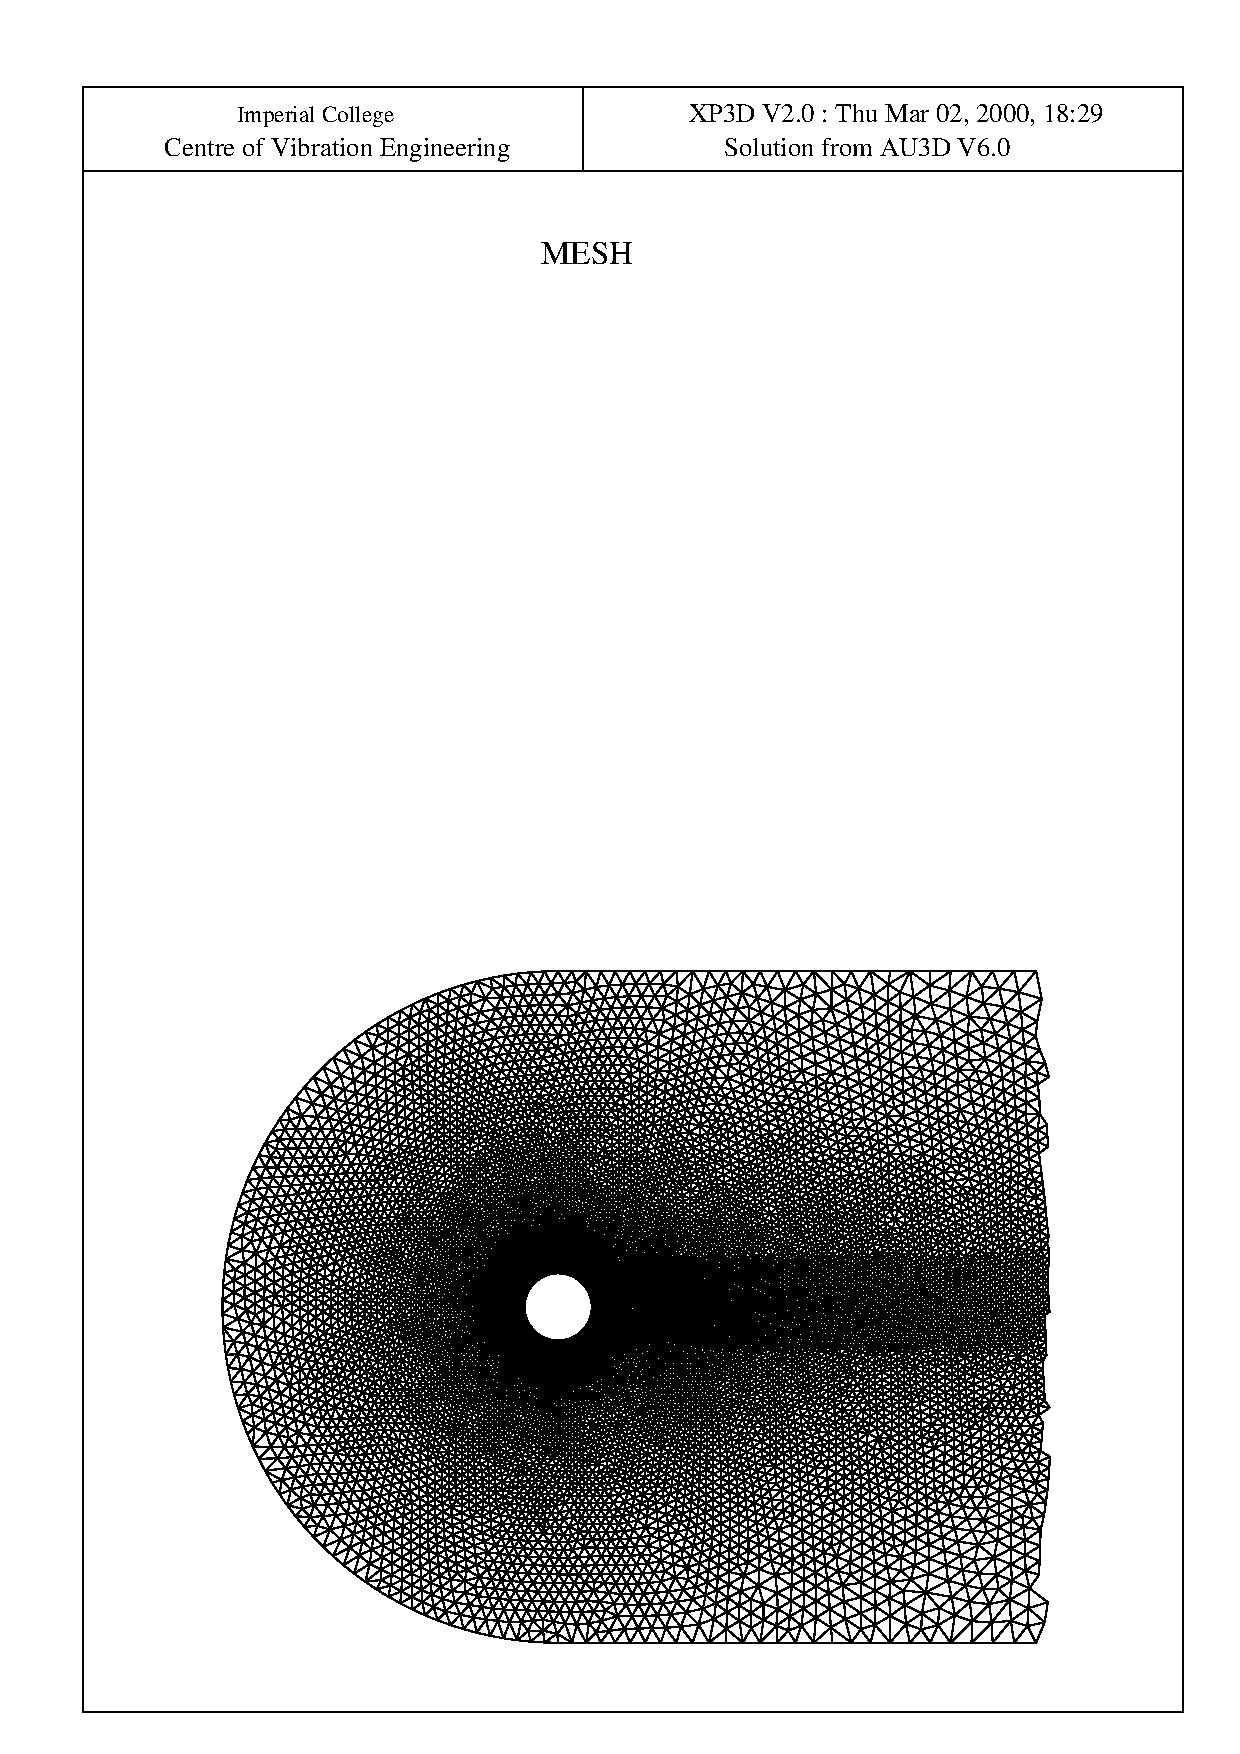
\includegraphics[height=60mm,clip=t]{CHAP_NONLIN/FIGURE/cil_me1.pdf}}
        &
    \subfigure[Zoom view at leading edge]
        {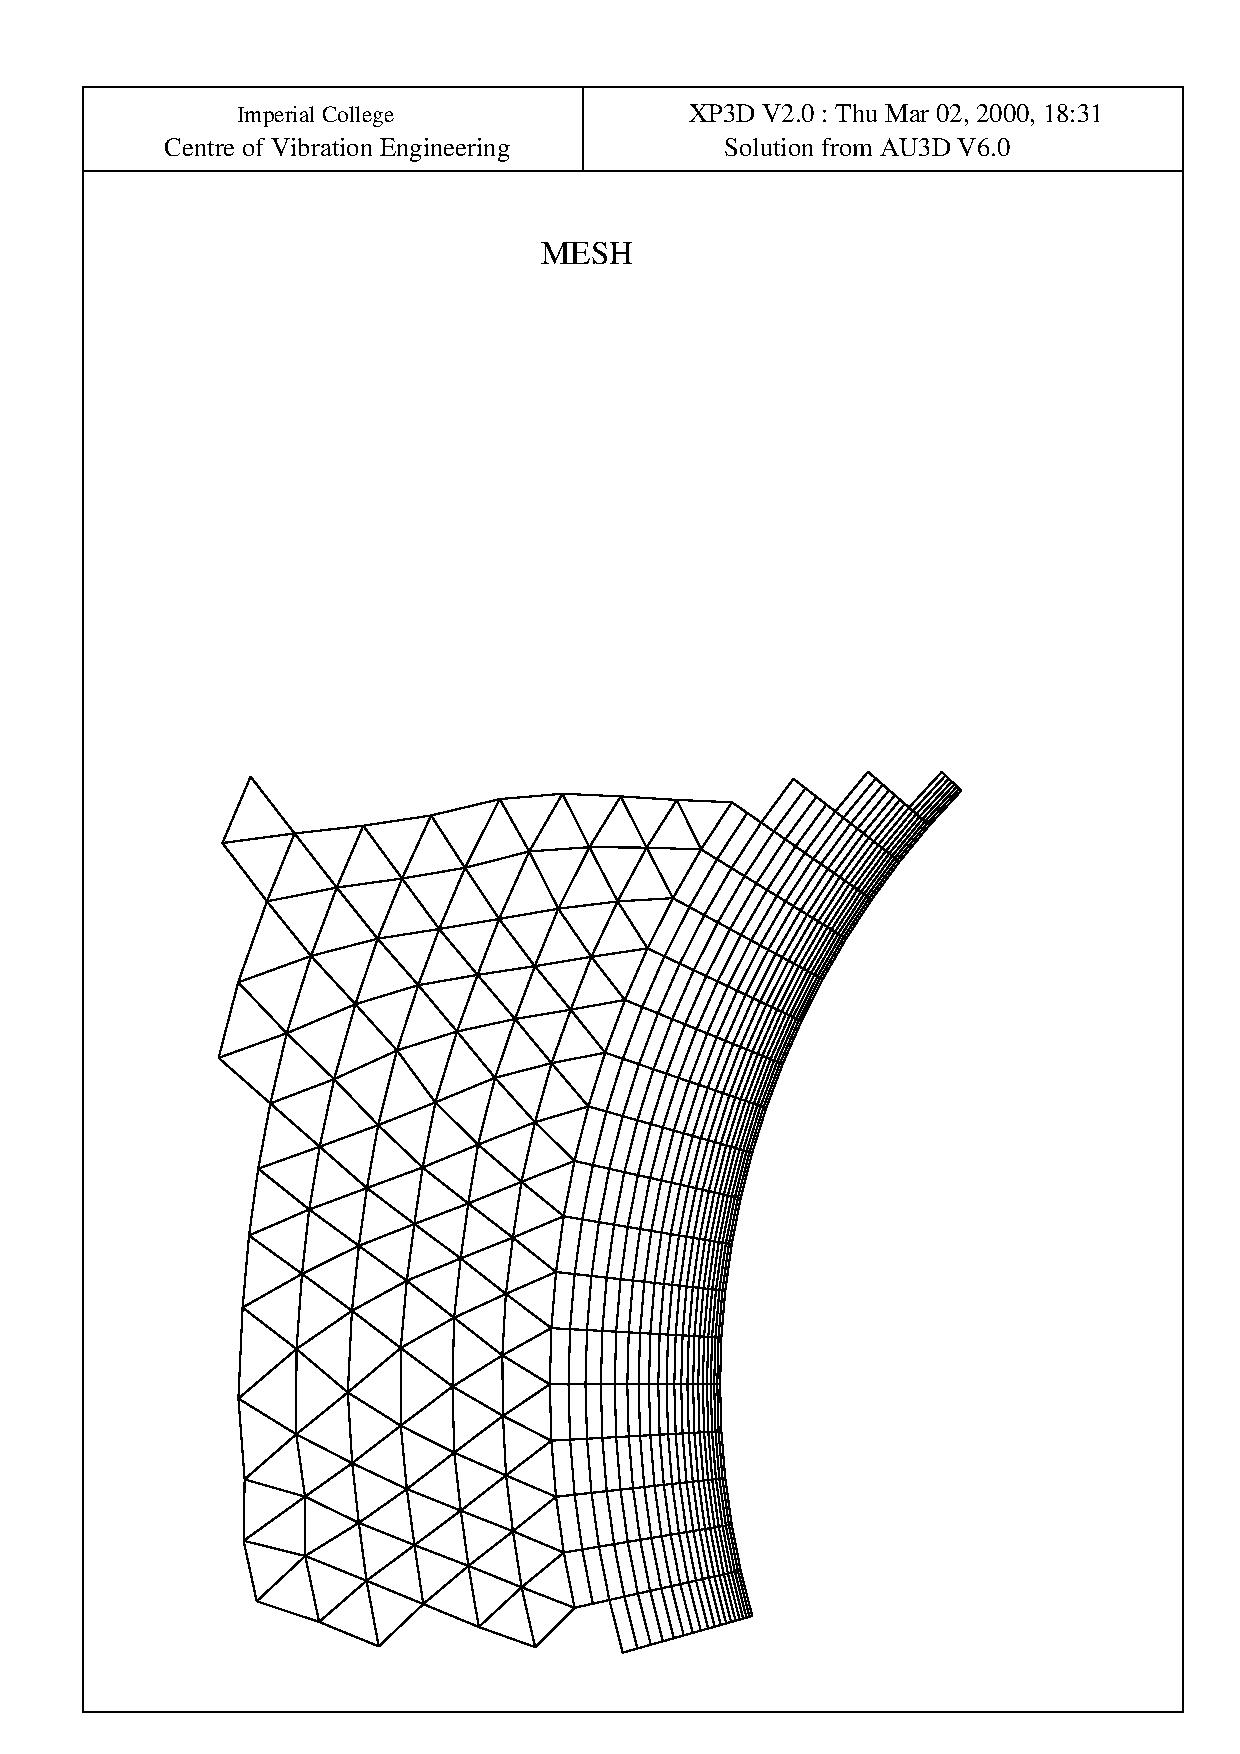
\includegraphics[height=60mm,clip=t]{CHAP_NONLIN/FIGURE/cil_me0.pdf}}
  \end{tabular}
 \end{center}
 \vspace{-5mm}
 \caption{Circular cylinder. Computational mesh}
 \label{cil_mesh1.fig}
\end{figure}
%
 This test case is intended to predict the natural vortex shedding
 past a cylinder in a laminar incompressible flow regime.
 Vortex shedding is one of many viscous flows which, though posed
 with fixed and steady boundary conditions, evolve into unsteady
 motions because of flow instability.
 If one consider a circular cylinder with diameter $d$, then
 the incompressible flow field generated by a uniform
 velocity at infinity $u_\infty$
 is dependent solely upon the Reynolds number $Re_d$

%
\beq
  Re_d = \frac{\rho_\infty u_\infty d}{\mu_\infty}
\eeq
%
 If $Re_d < 40$ the flow is steady. If $Re_d > 40$
 the flow becomes unstable and consequently unsteady when
 $Re_d > 50$. The flow field is caracterised by a unsteady wake
 which consists of pairs of vortices shed alternately from the
 upper and lower part of the cylinder surface.
 If $50 < Re_d < 150$ such a wake structure is well organised and is
 called Karman vortex sheet after a paper by Karman (1911) explaining
 this alternation to be a stable configuration for vortex pairs
 (Schlichting \citeyearNP{Schlichting}).
 An important feature of this flow is that the dimensionless
 cylinder frequency or Stroudal number

%
\beq
  St = \frac{f d}{u_\infty}
\eeq
%
 remains constant $\approx 0.21$ for $100 < Re_d < 10,000$. Thus, in this
 Reynolds number range, the shedding cycle takes place during the time
 that the free-stream moves approximately five cylinder diameters.
%
\begin{figure}[ht]
 \begin{center}
  \begin{tabular}{ccc}
    \subfigure[Grid 2: 4308 cells]
       {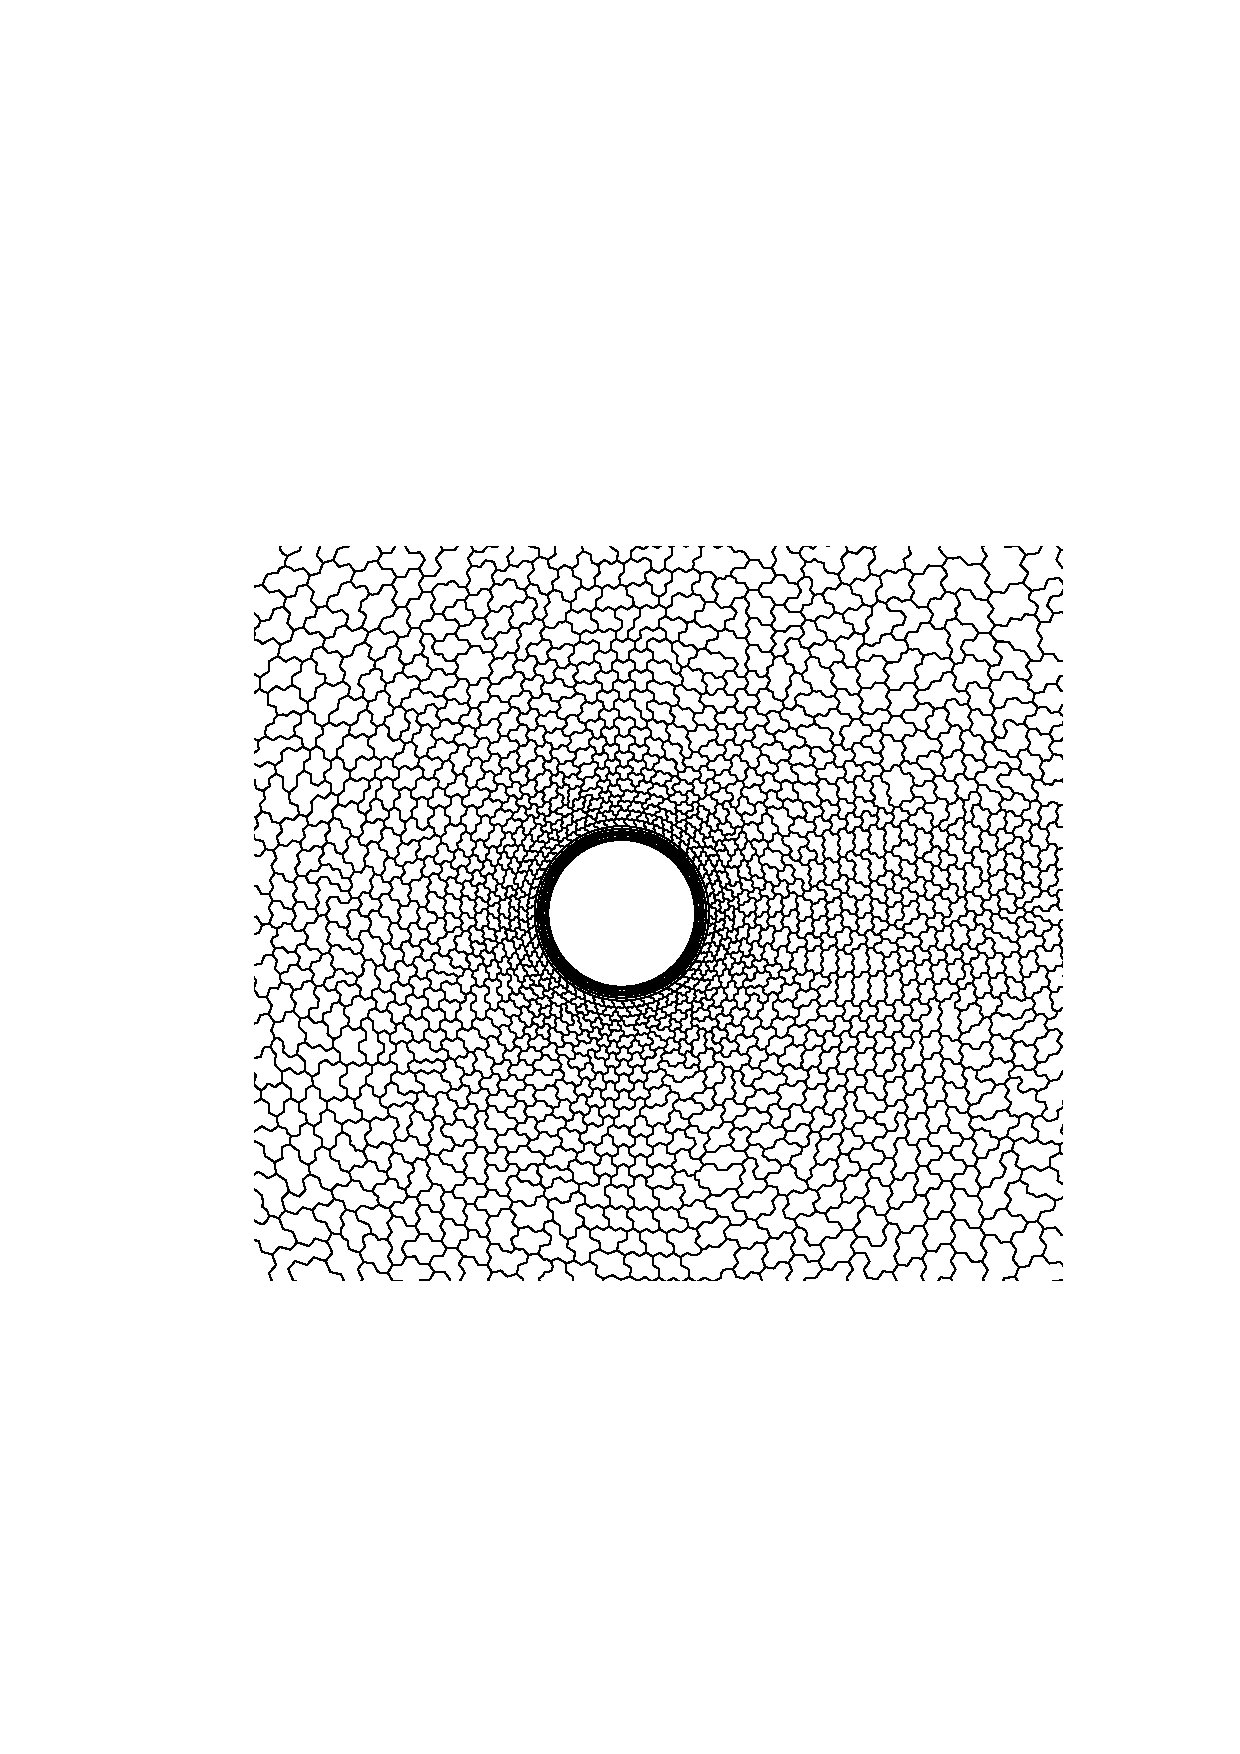
\includegraphics[width=45mm,clip=t]{CHAP_NONLIN/FIGURE/cil_me2.pdf}}
        &
    \subfigure[Grid 3: 1095 cells]
       {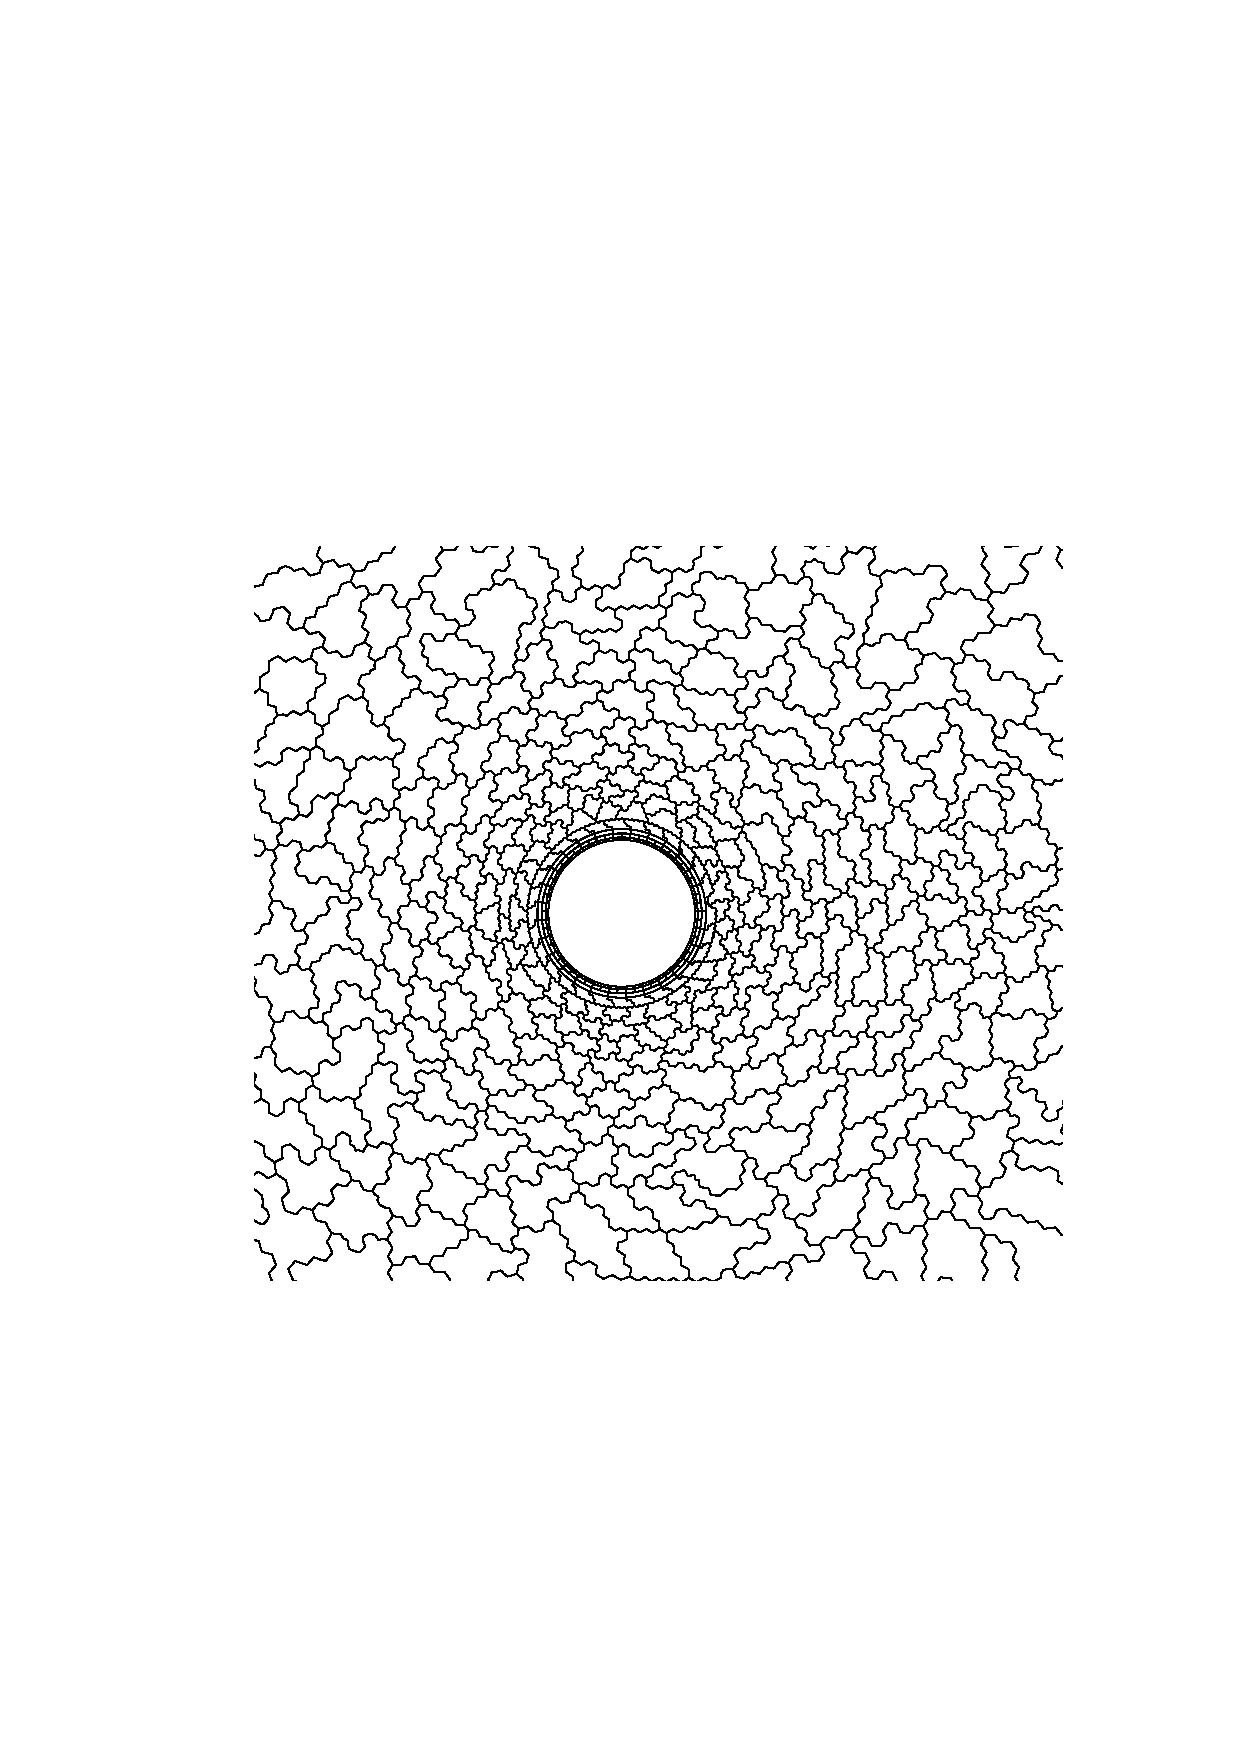
\includegraphics[width=45mm,clip=t]{CHAP_NONLIN/FIGURE/cil_me3.pdf}}
        &
    \subfigure[Grid 4: 283 cells]
       {\includegraphics[width=45mm,clip=t]{CHAP_NONLIN/FIGURE/cil_me4.pdf}}
  \end{tabular}
 \end{center}
 \vspace{-5mm}
 \caption{Circular cylinder. Agglomerated grids}
 \label{cil_mesh2.fig}
\end{figure}

 Fig. \ref{cil_mesh1.fig} shows the computational mesh used for this test case,
 it contains 2280 quadrilaterals in the boundary layer and 29863
 triangles in the rest of the domain for a total number of point of 17391.
 Fig. \ref{cil_mesh2.fig} shows the three agglomerated grids used in the time
 accurate multigrid algorithm.
 Four different calculations were performed for various Reynolds numbers
 with an inlet Mach number of 0.2
 and the computed Stroudal number is reported in Fig. \ref{stroudal.fig}a together
 with the experimental value of 0.21. The comparison is satisfactory for
 all four test cases.
 Fig. \ref{stroudal.fig}b reports the evolution in time of the pressure coefficient
 at a point in the wake close to the cylinder. The time history refers to three cycles of
 oscillations after a periodic flow conditions is reached. The very periodic behaviour
 of the flow is evident and proves the robustness and accuracy of the scheme.
%
\begin{figure}
 \begin{center}
  \begin{tabular}{c}
    \subfigure[Computed Stroudal number]
       {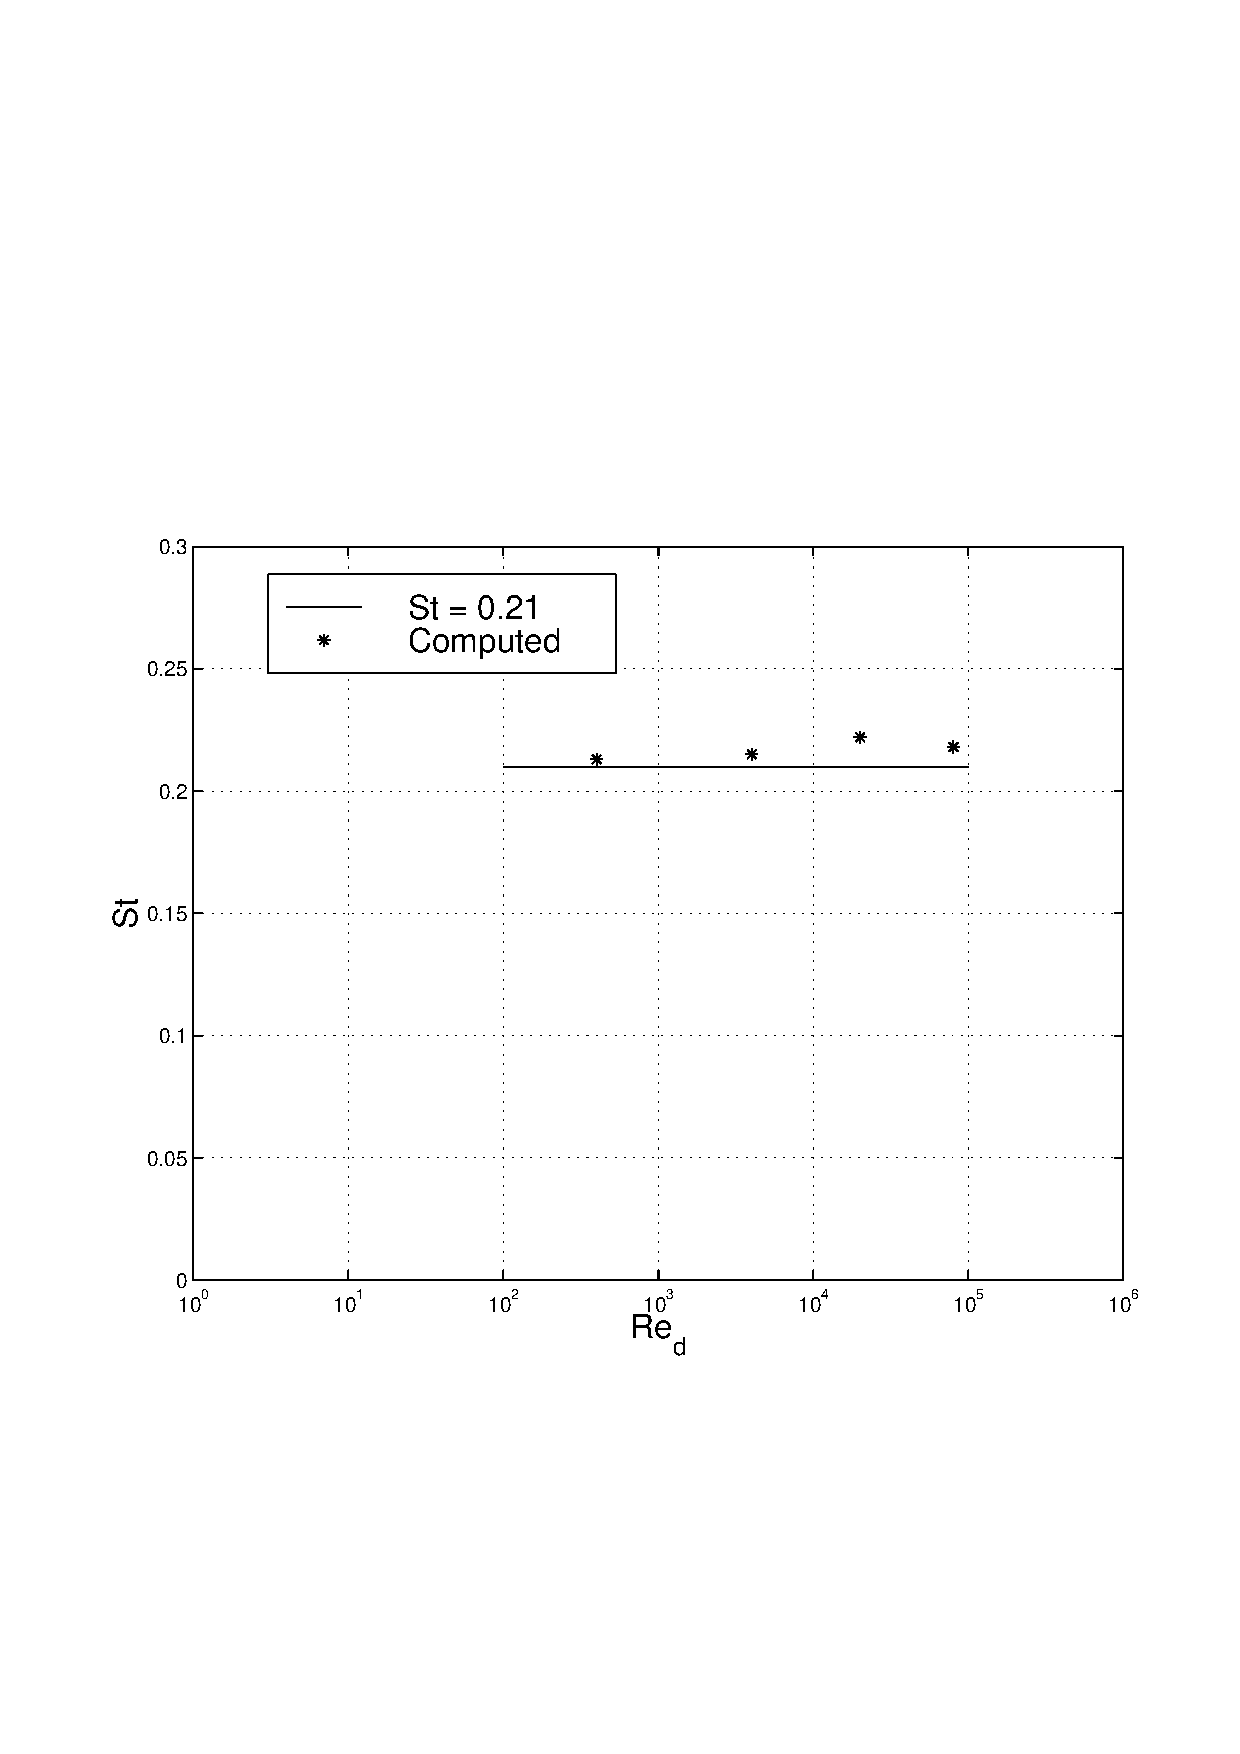
\includegraphics[width=110mm,clip=t]{CHAP_NONLIN/FIGURE/stroud.pdf}}
        \\
    \subfigure[$c_p$ evolution]
       {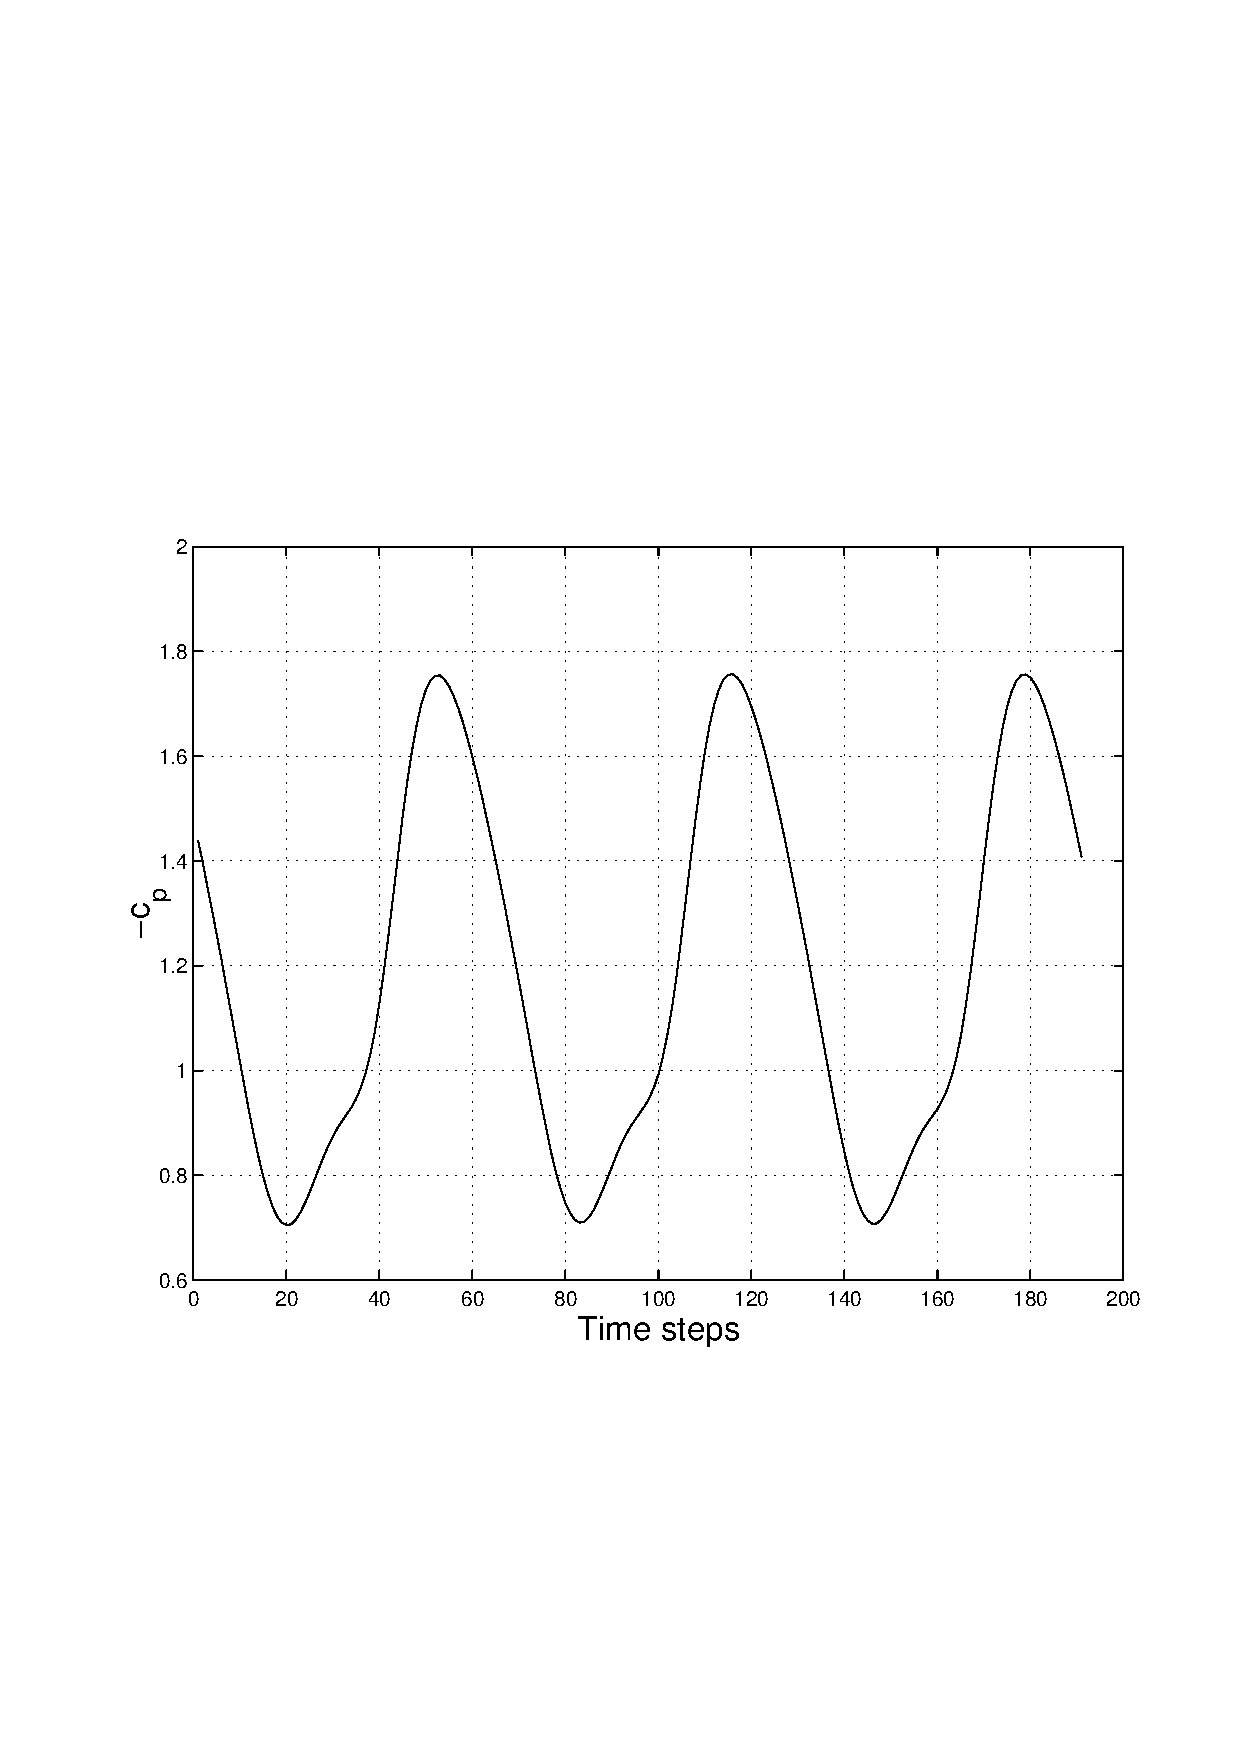
\includegraphics[width=110mm,clip=t]{CHAP_NONLIN/FIGURE/prehis.pdf}}
  \end{tabular}
 \end{center}
 \vspace{-5mm}
 \caption{Circular cylinder. Computed Stroudal number and $c_p$ evolution}
 \label{stroudal.fig}
\end{figure}
%

 The time step for those calculations was set to have 50 divisions over a cycle.
 This correspond to a local CFL number between two in the far field and three
 thousand in the boundary layer region.
%
\begin{figure}[ht]
 \begin{center}
  \begin{tabular}{c}
    \subfigure[$Re_d = 400$]
       {\begin{tabular}{ccc}
         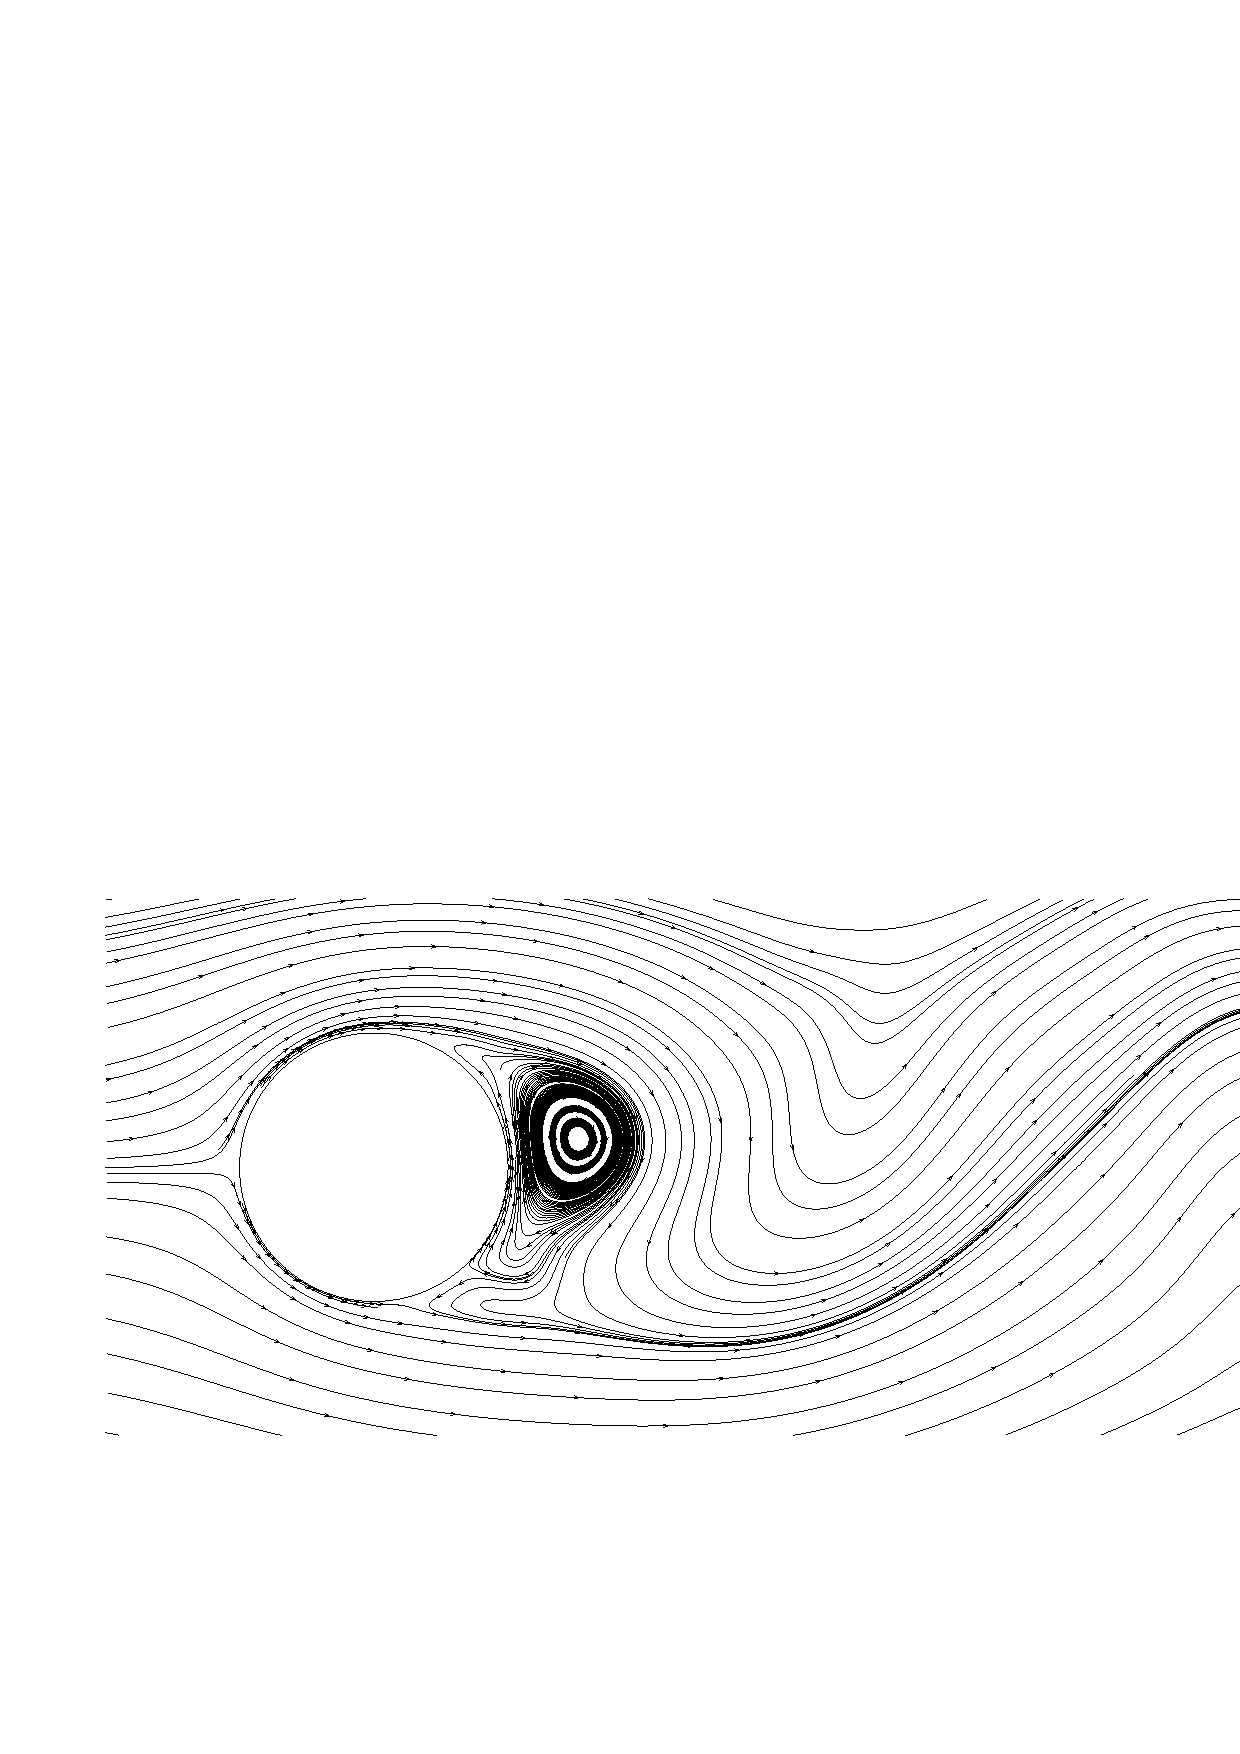
\includegraphics[width=45mm,clip=t]{CHAP_NONLIN/FIGURE/cil2.pdf}
         &
         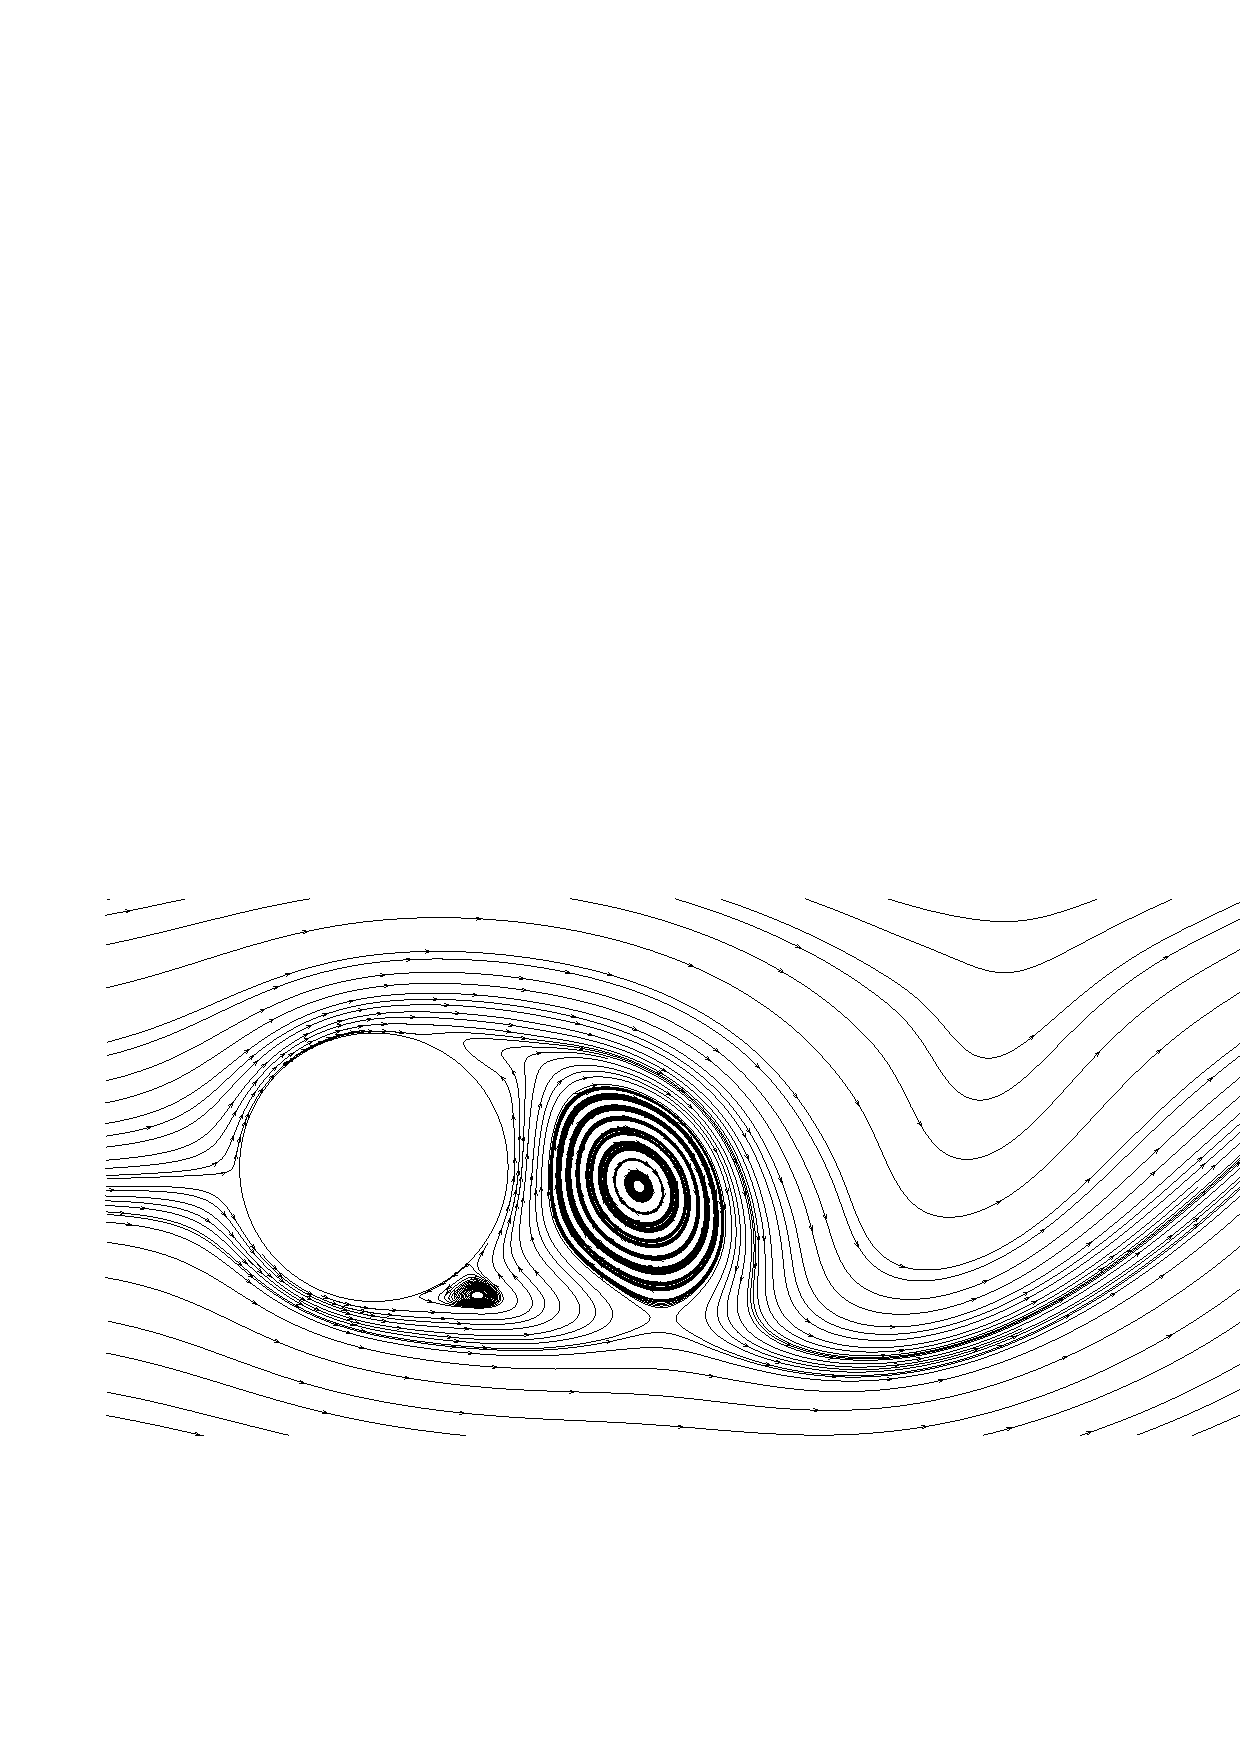
\includegraphics[width=45mm,clip=t]{CHAP_NONLIN/FIGURE/cil3.pdf}
         &
         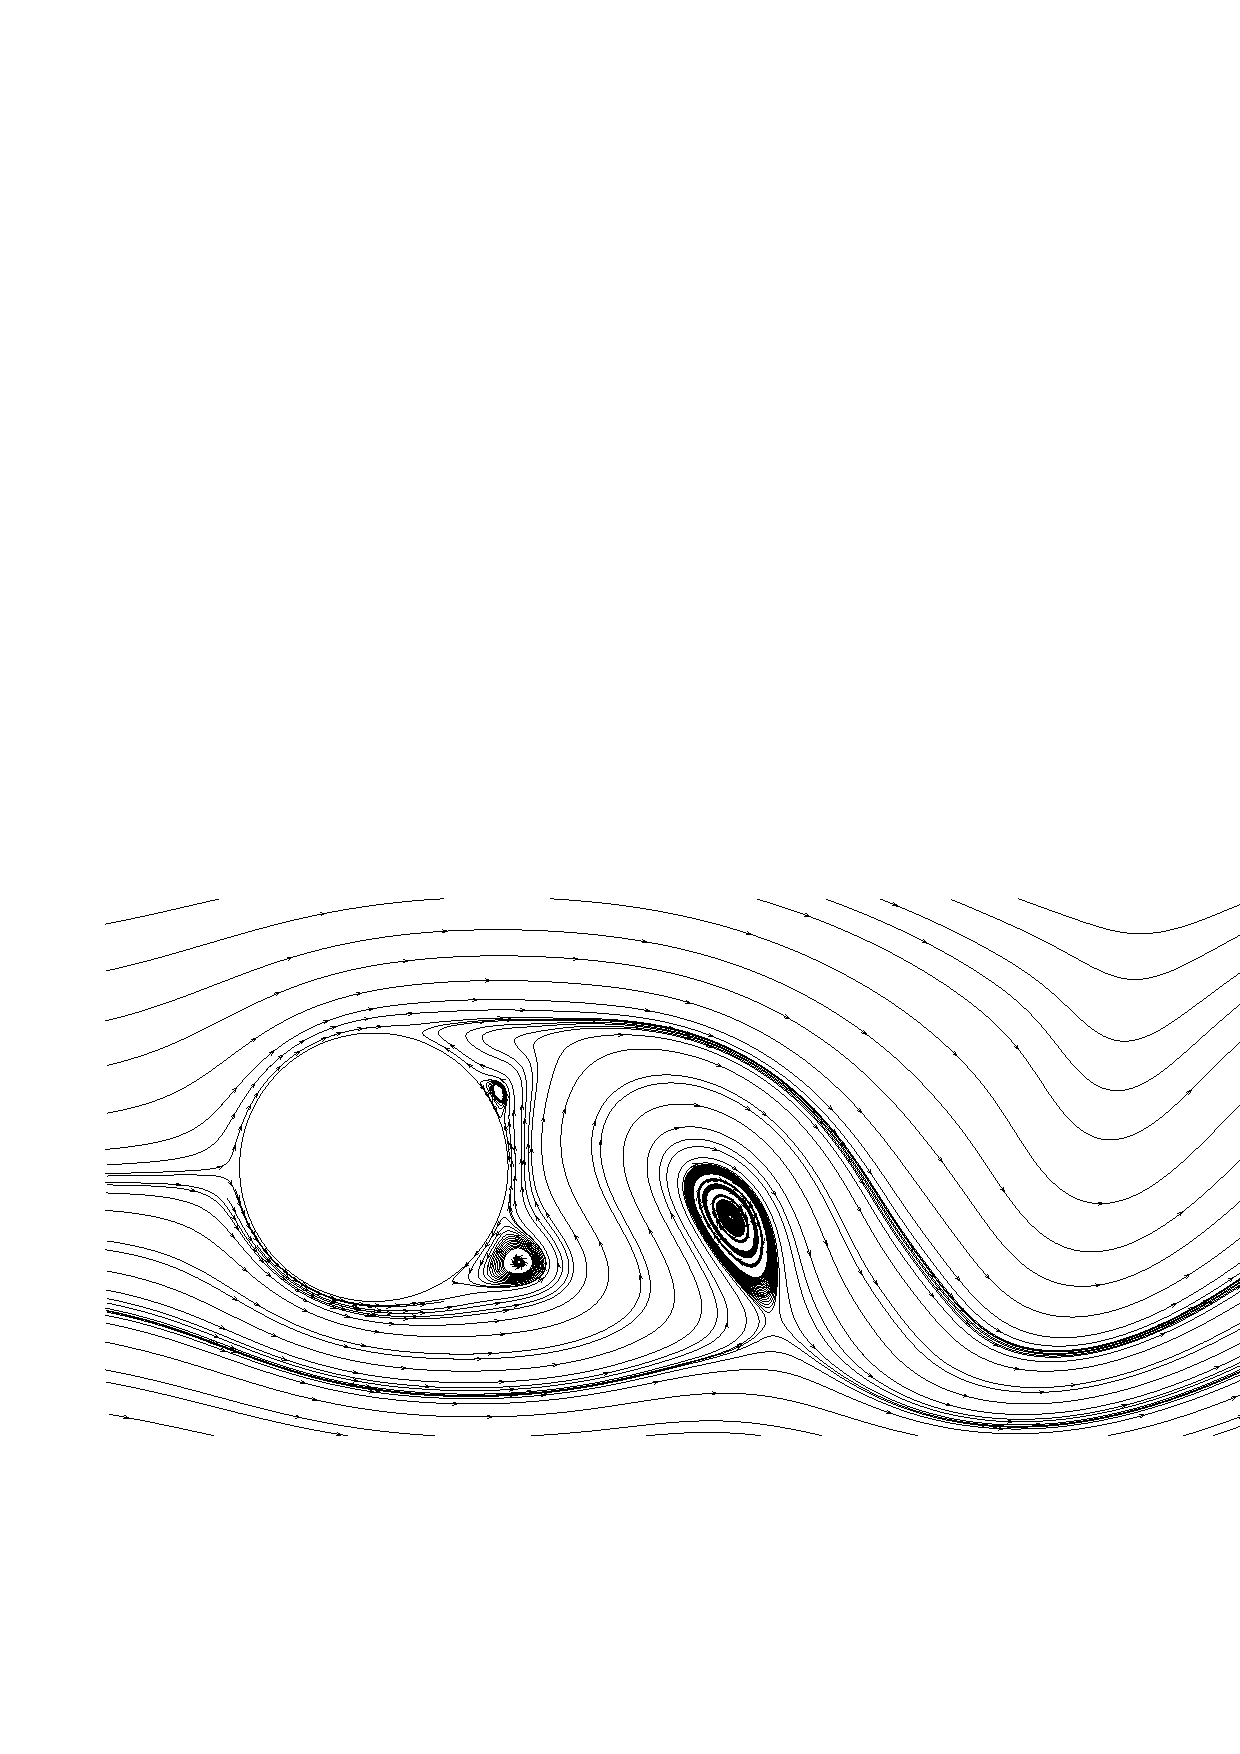
\includegraphics[width=45mm,clip=t]{CHAP_NONLIN/FIGURE/cil4.pdf}
        \\
         Time 1 & Time 2 & Time 3
        \\
         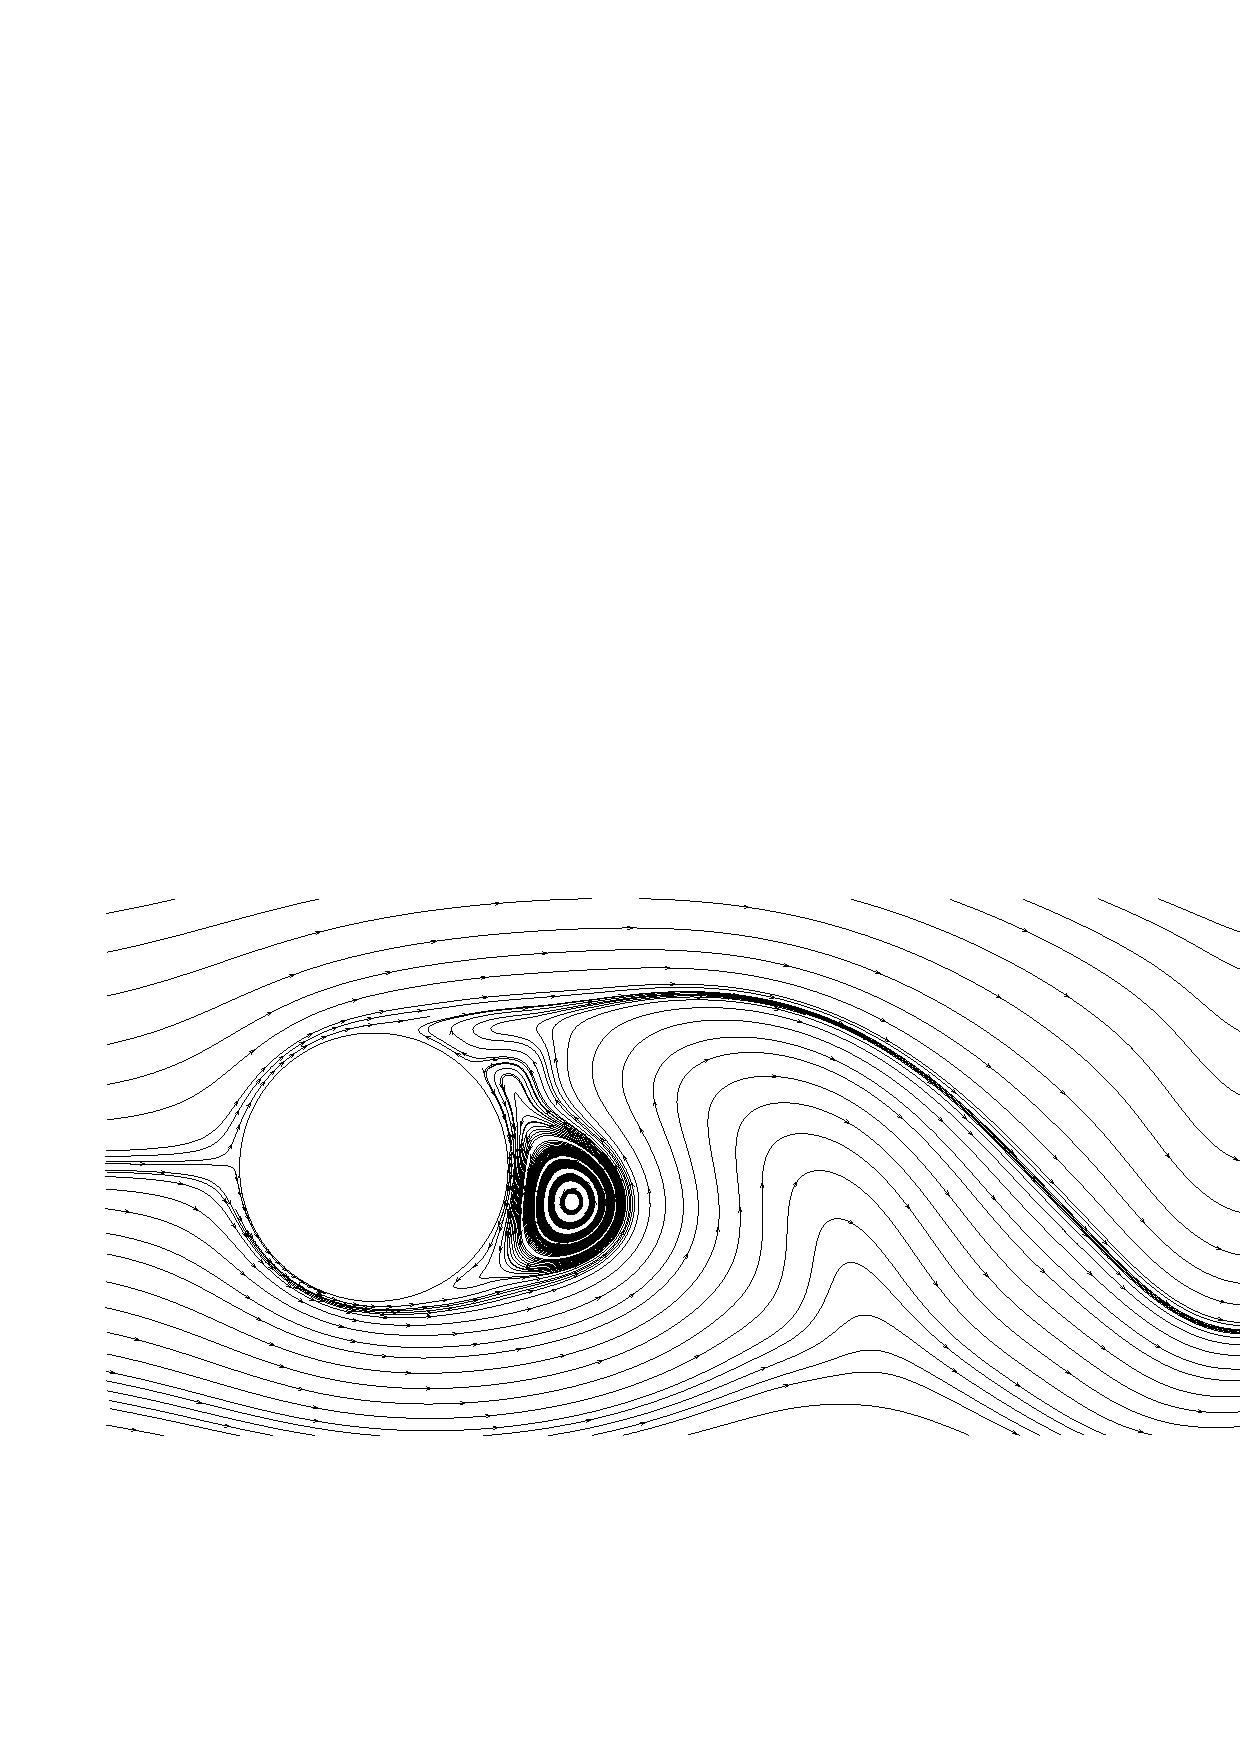
\includegraphics[width=45mm,clip=t]{CHAP_NONLIN/FIGURE/cil5.pdf}
         &
         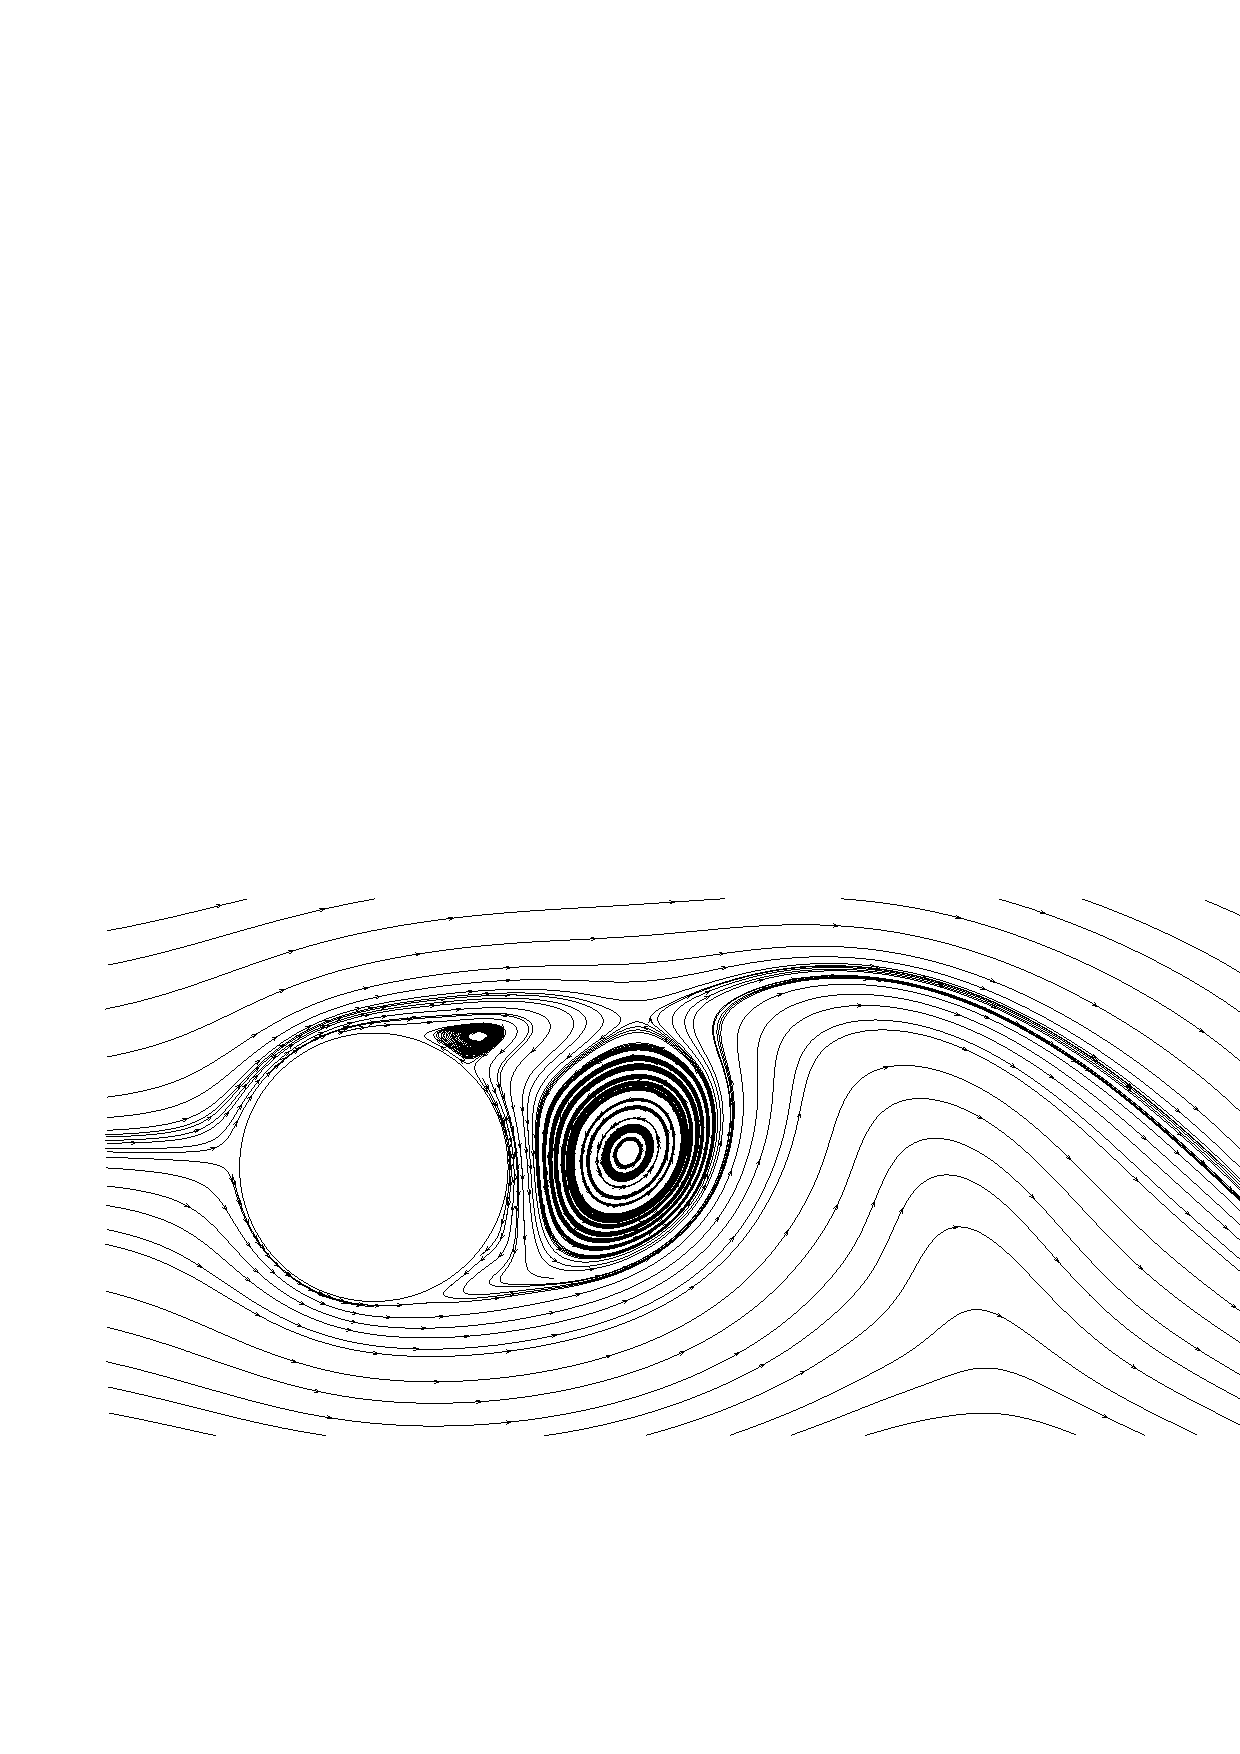
\includegraphics[width=45mm,clip=t]{CHAP_NONLIN/FIGURE/cil6.pdf}
         &
         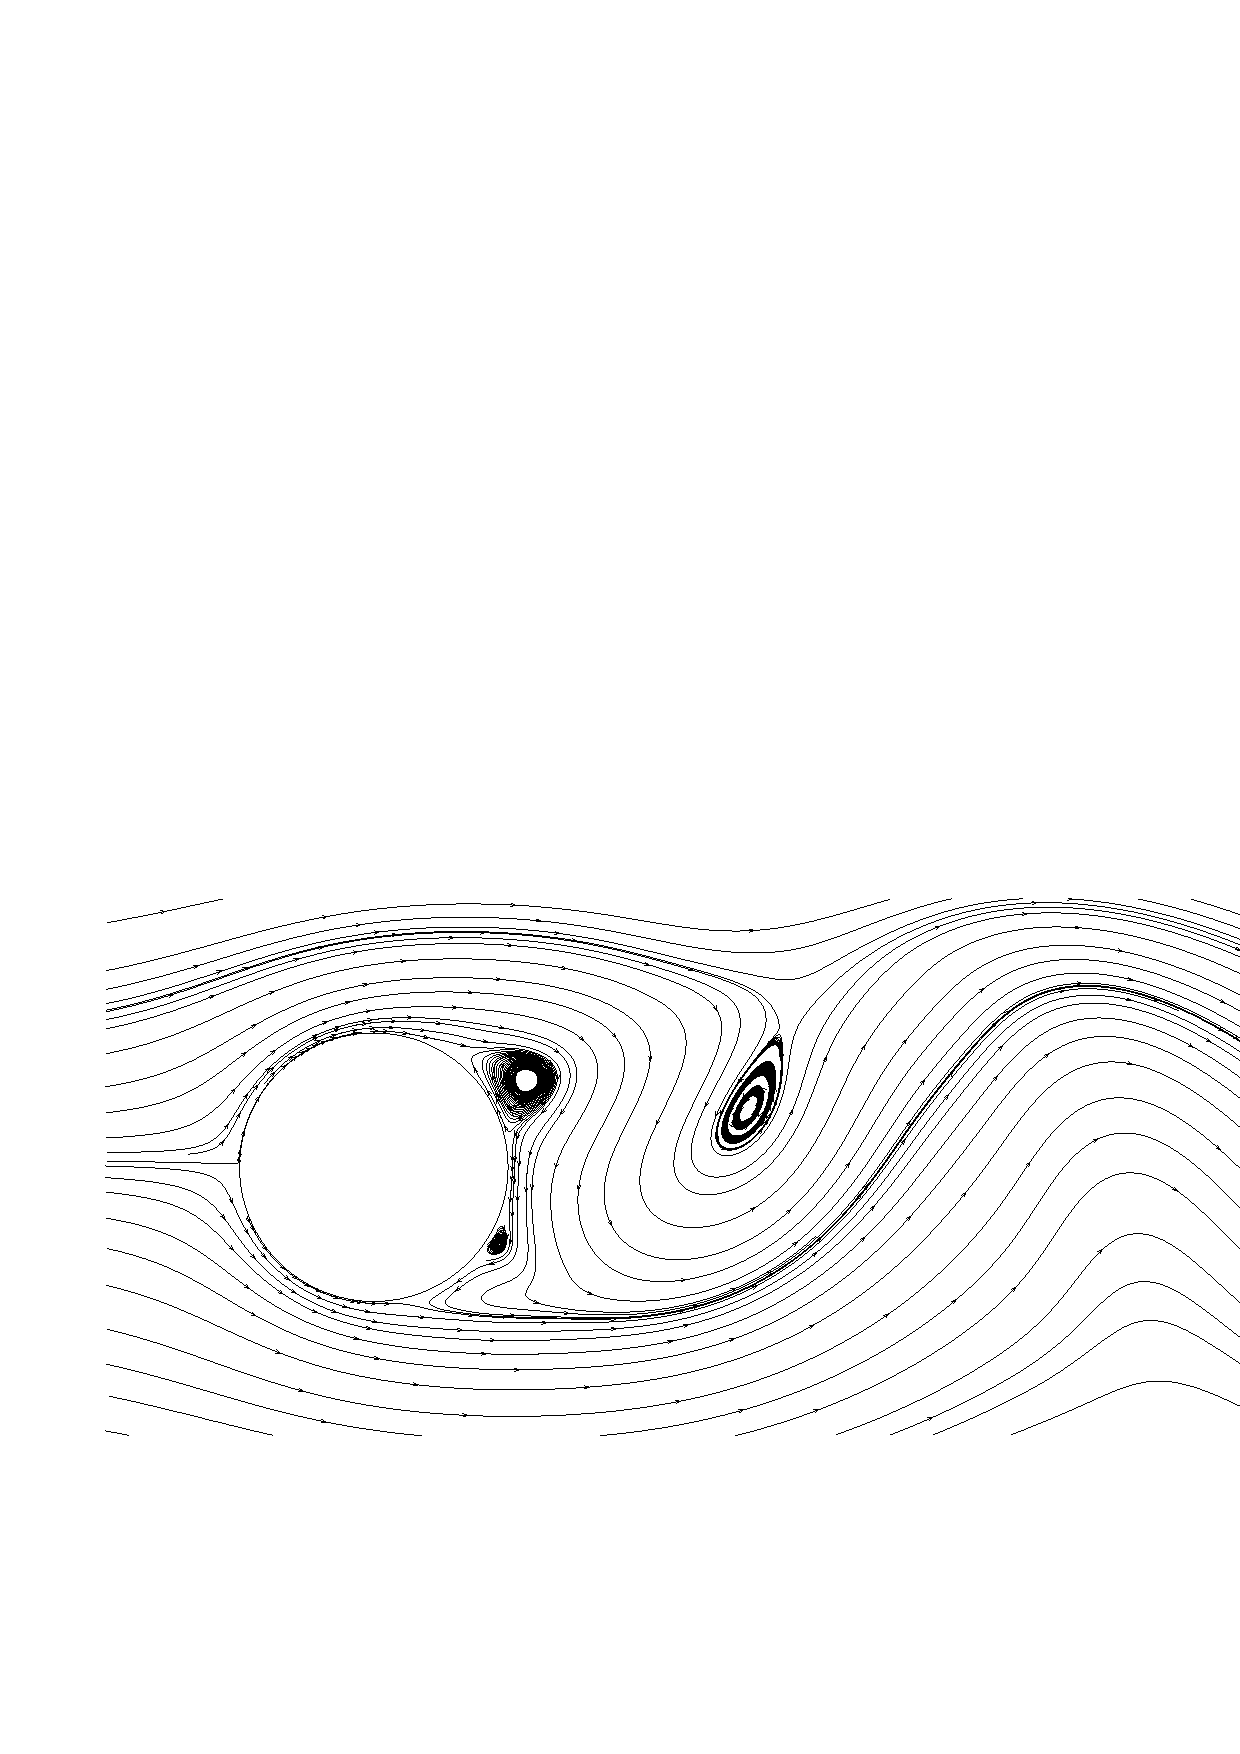
\includegraphics[width=45mm,clip=t]{CHAP_NONLIN/FIGURE/cil1.pdf}
        \\
         Time 4 & Time 5 & Time 6
       \end{tabular}}
     \\
    \subfigure[$Re_d = 4000$]
       {\begin{tabular}{ccc}
         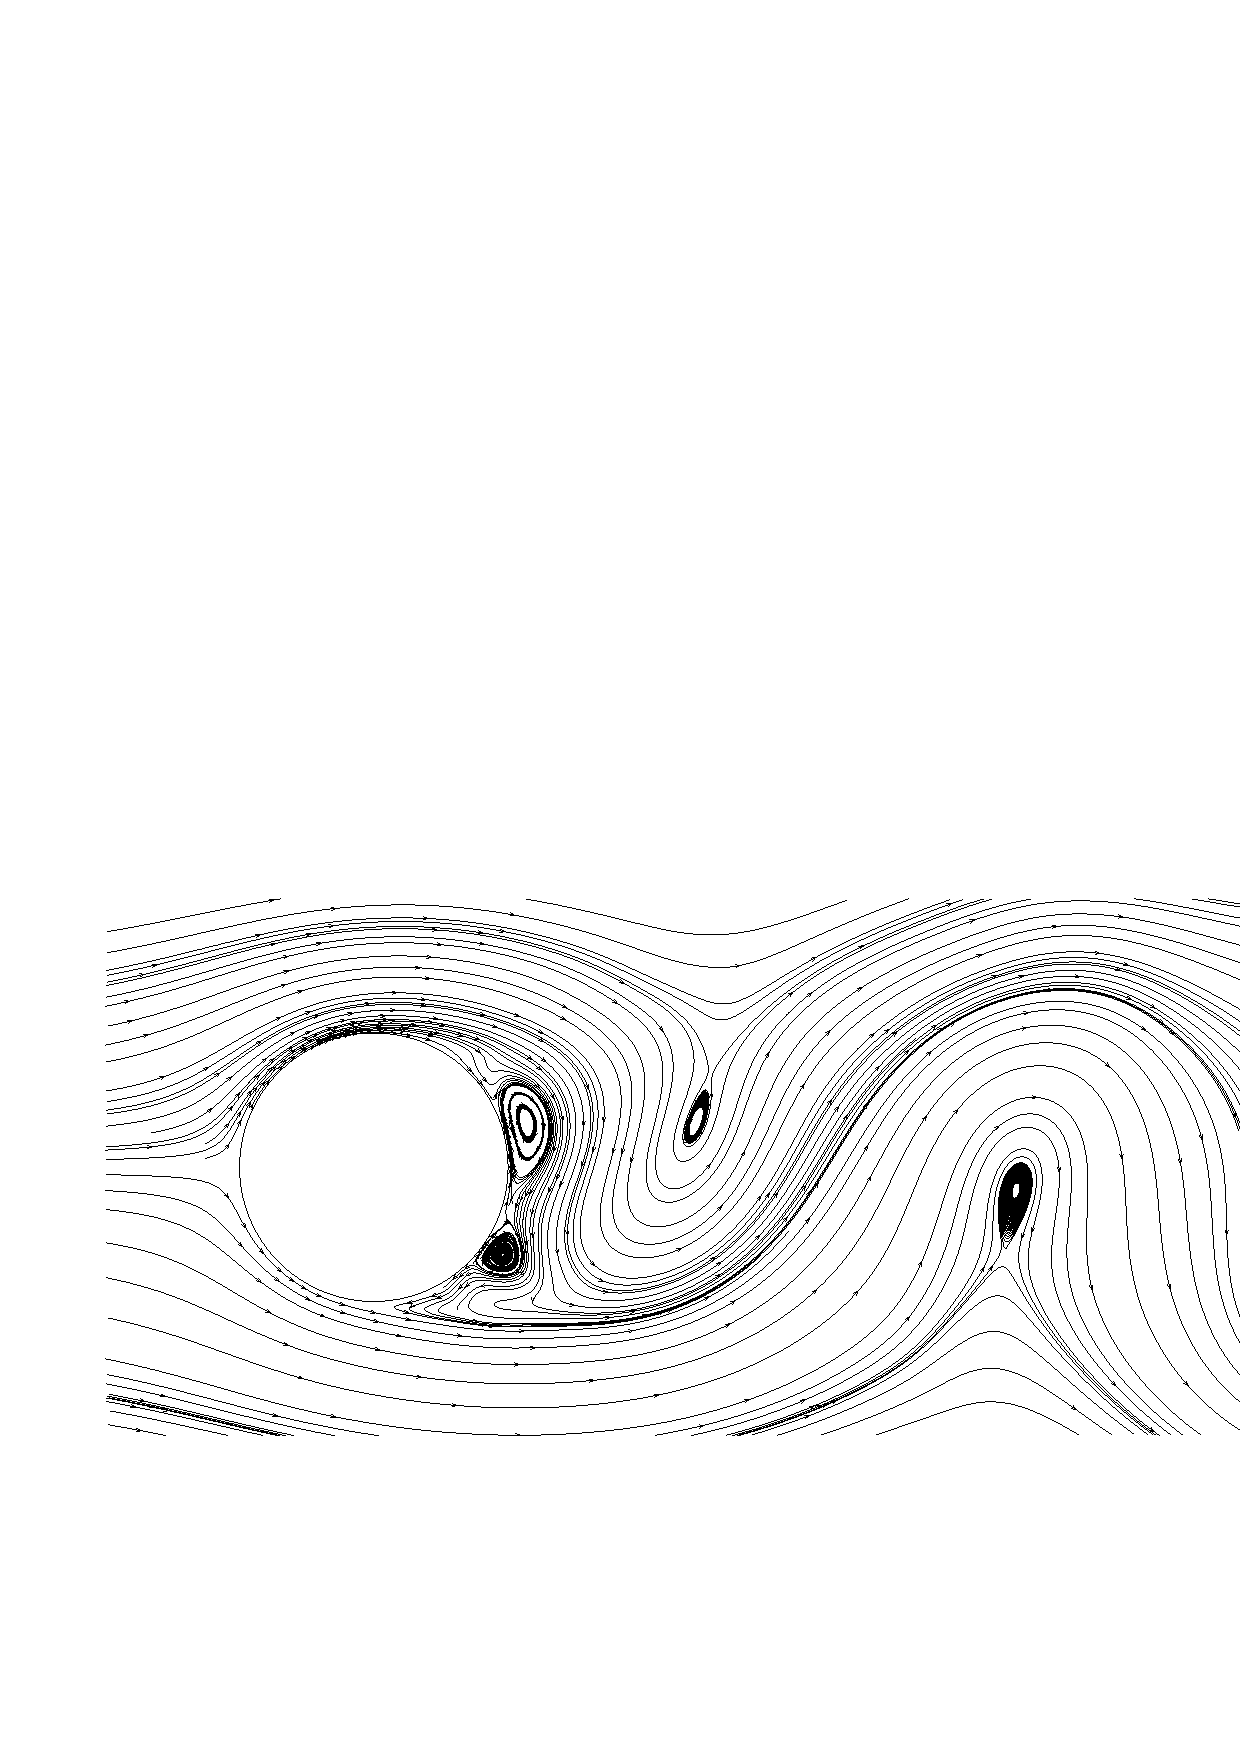
\includegraphics[width=45mm,clip=t]{CHAP_NONLIN/FIGURE/cim2.pdf}
         &
         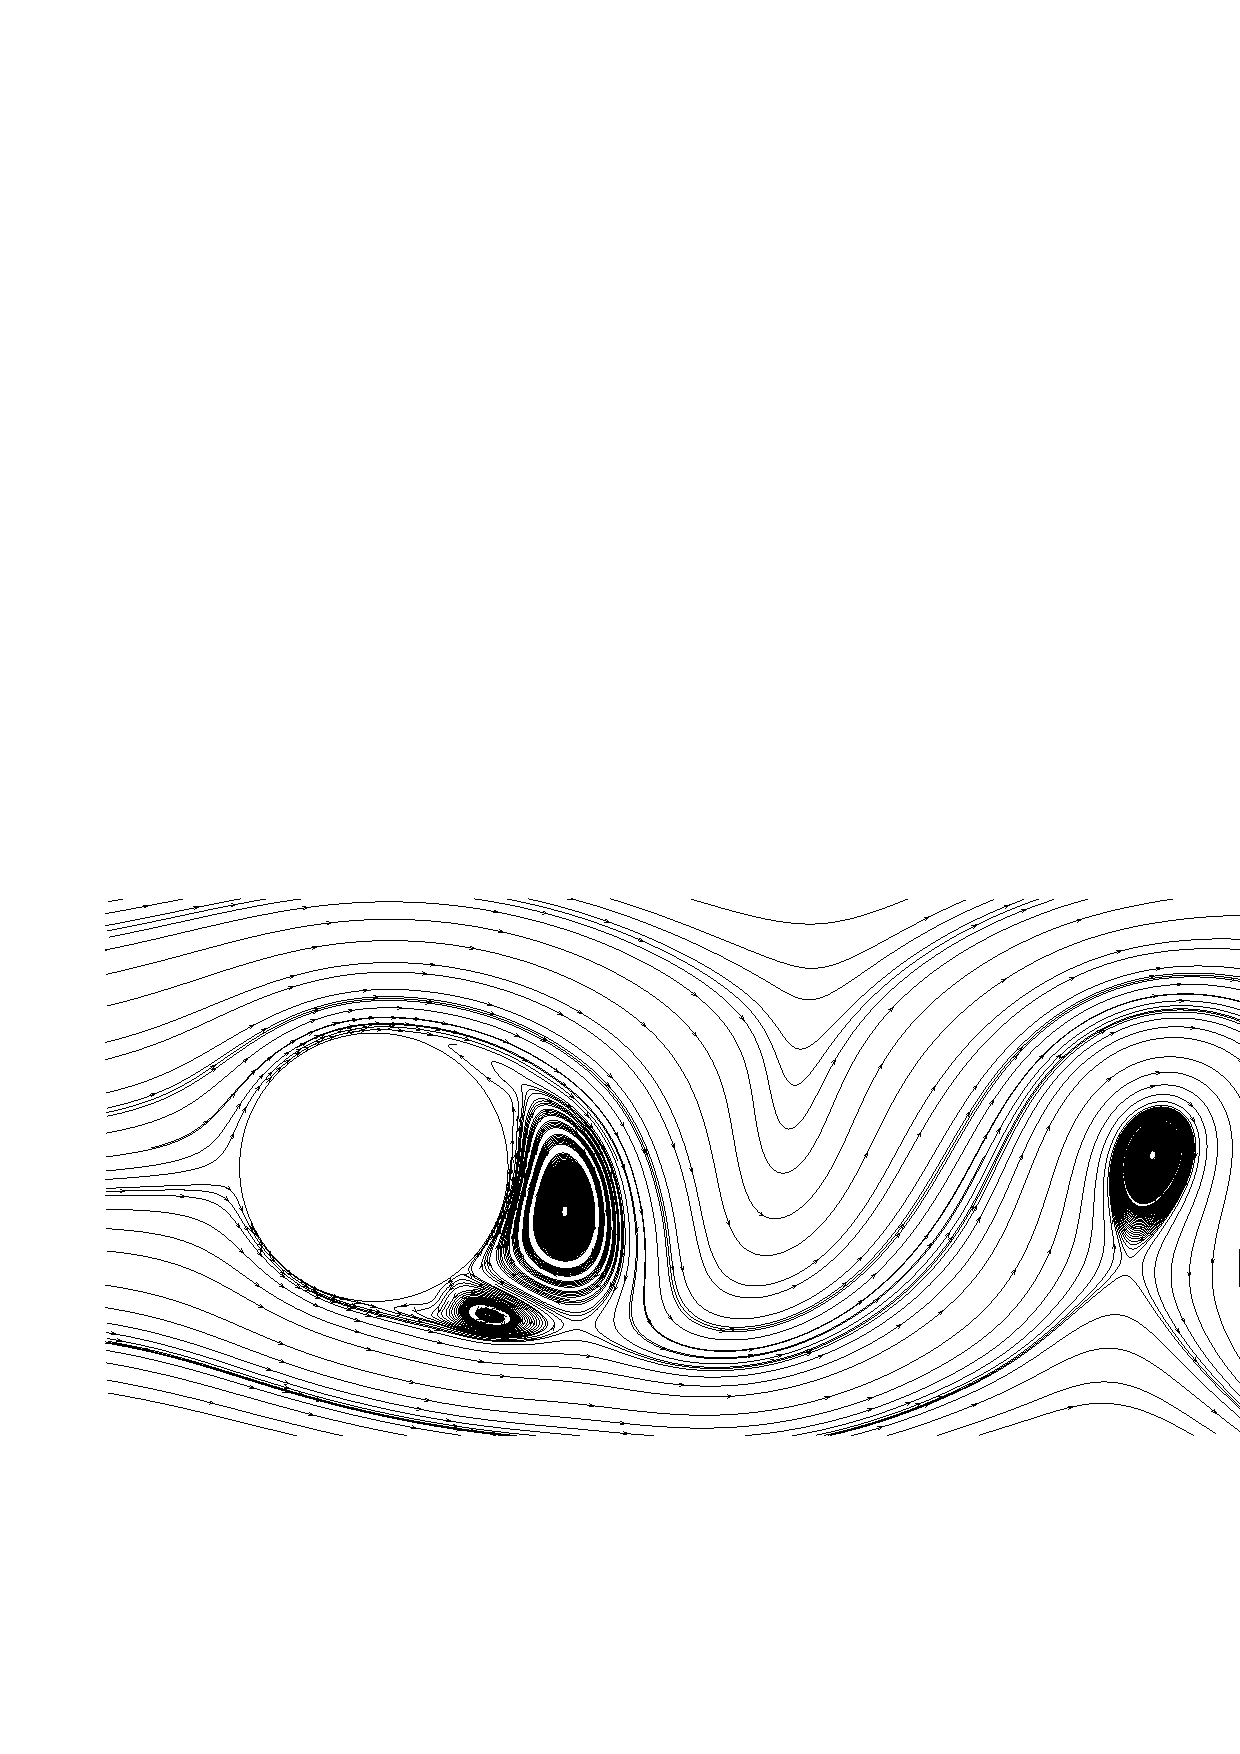
\includegraphics[width=45mm,clip=t]{CHAP_NONLIN/FIGURE/cim3.pdf}
         &
         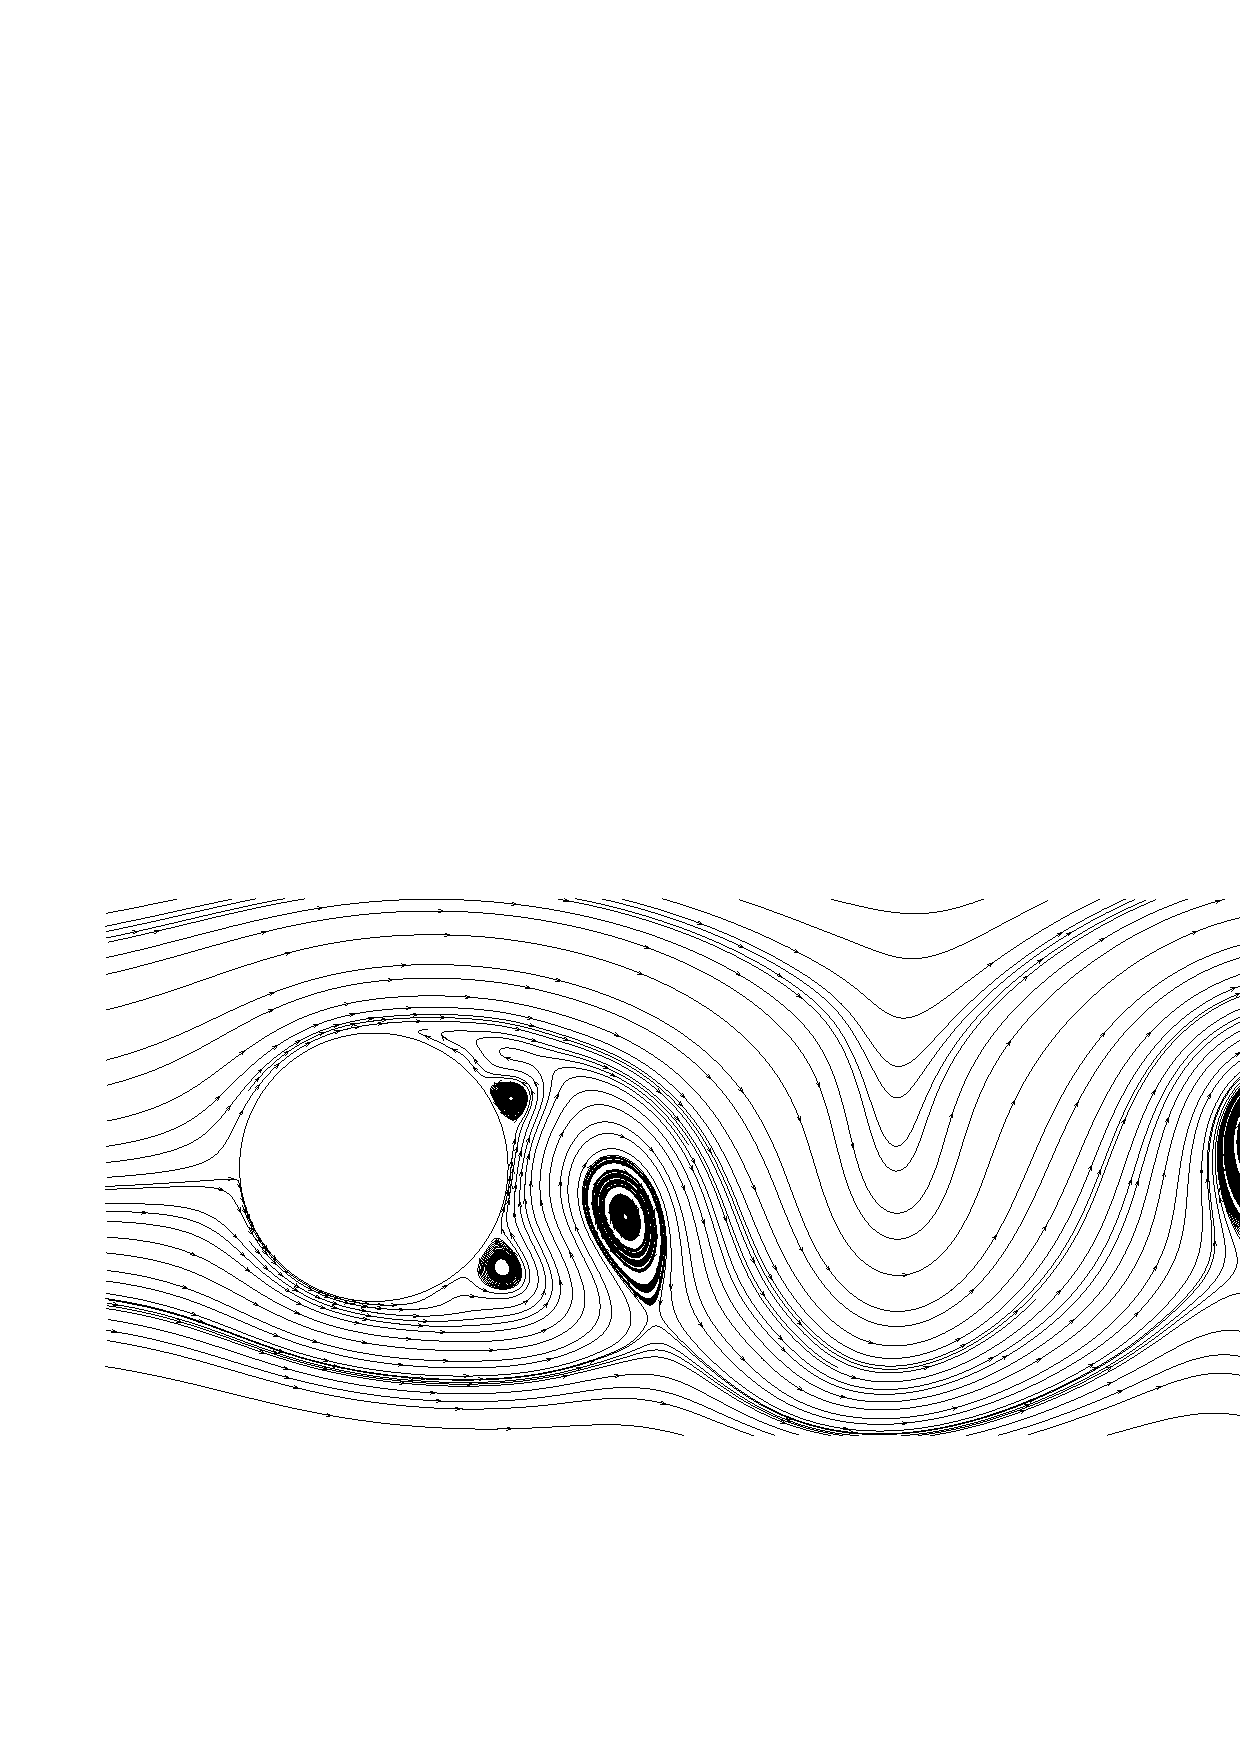
\includegraphics[width=45mm,clip=t]{CHAP_NONLIN/FIGURE/cim4.pdf}
        \\
         Time 1 & Time 2 & Time 3
        \\
         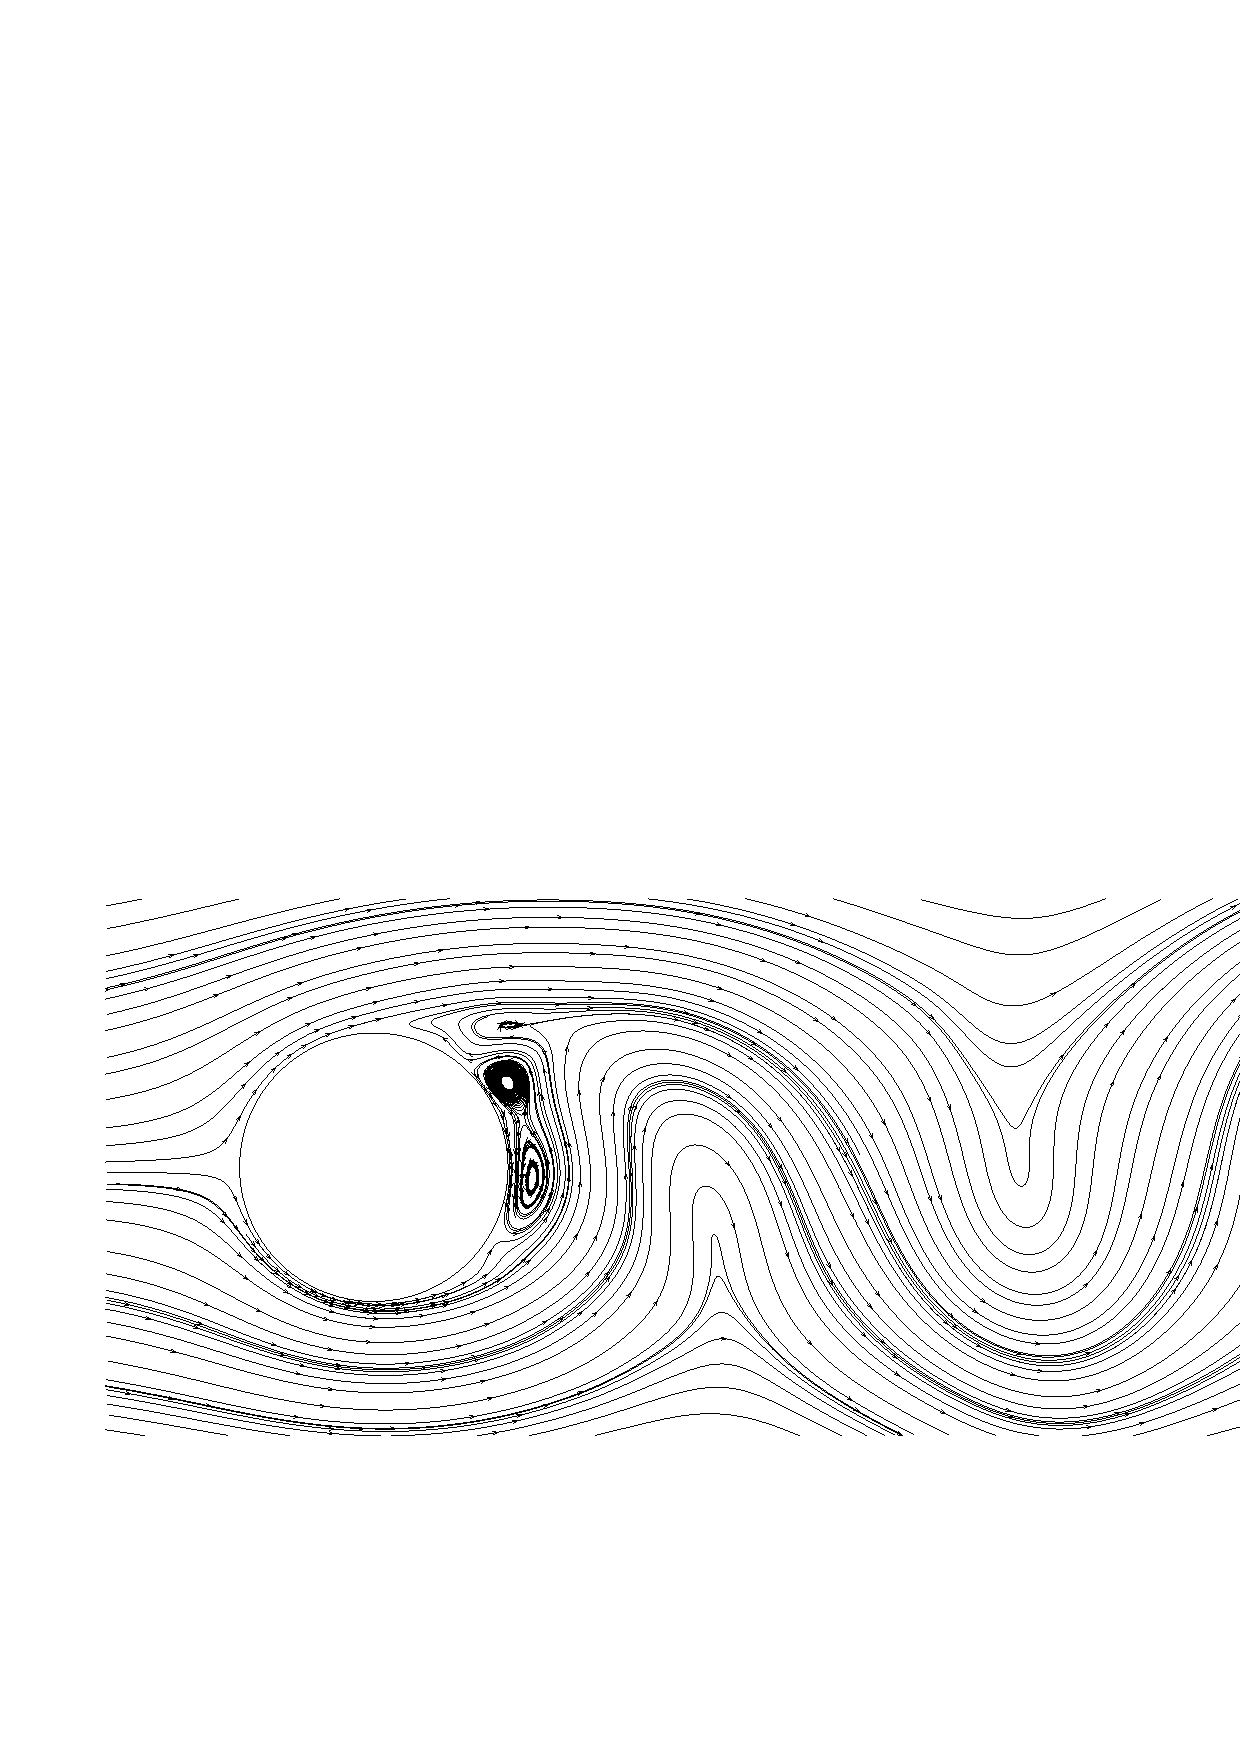
\includegraphics[width=45mm,clip=t]{CHAP_NONLIN/FIGURE/cim5.pdf}
         &
         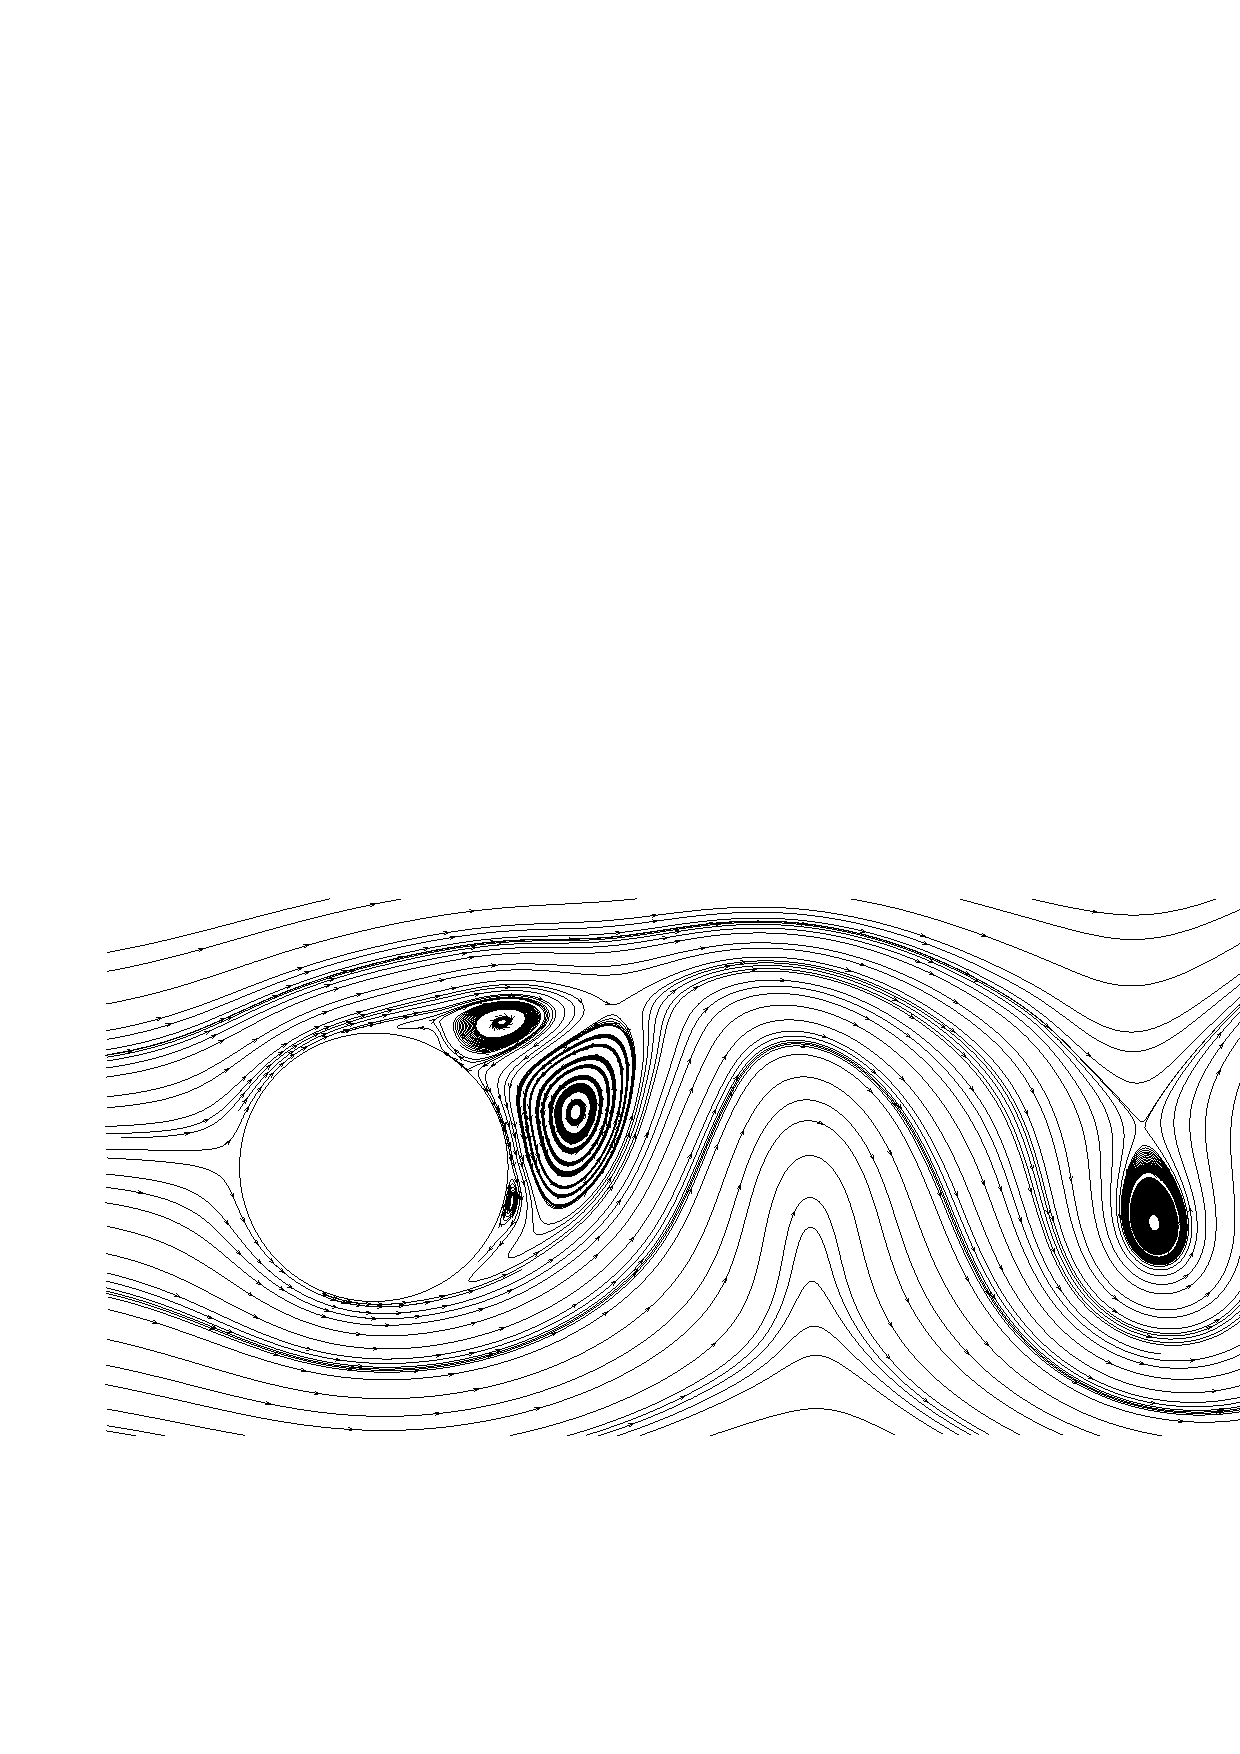
\includegraphics[width=45mm,clip=t]{CHAP_NONLIN/FIGURE/cim6.pdf}
         &
         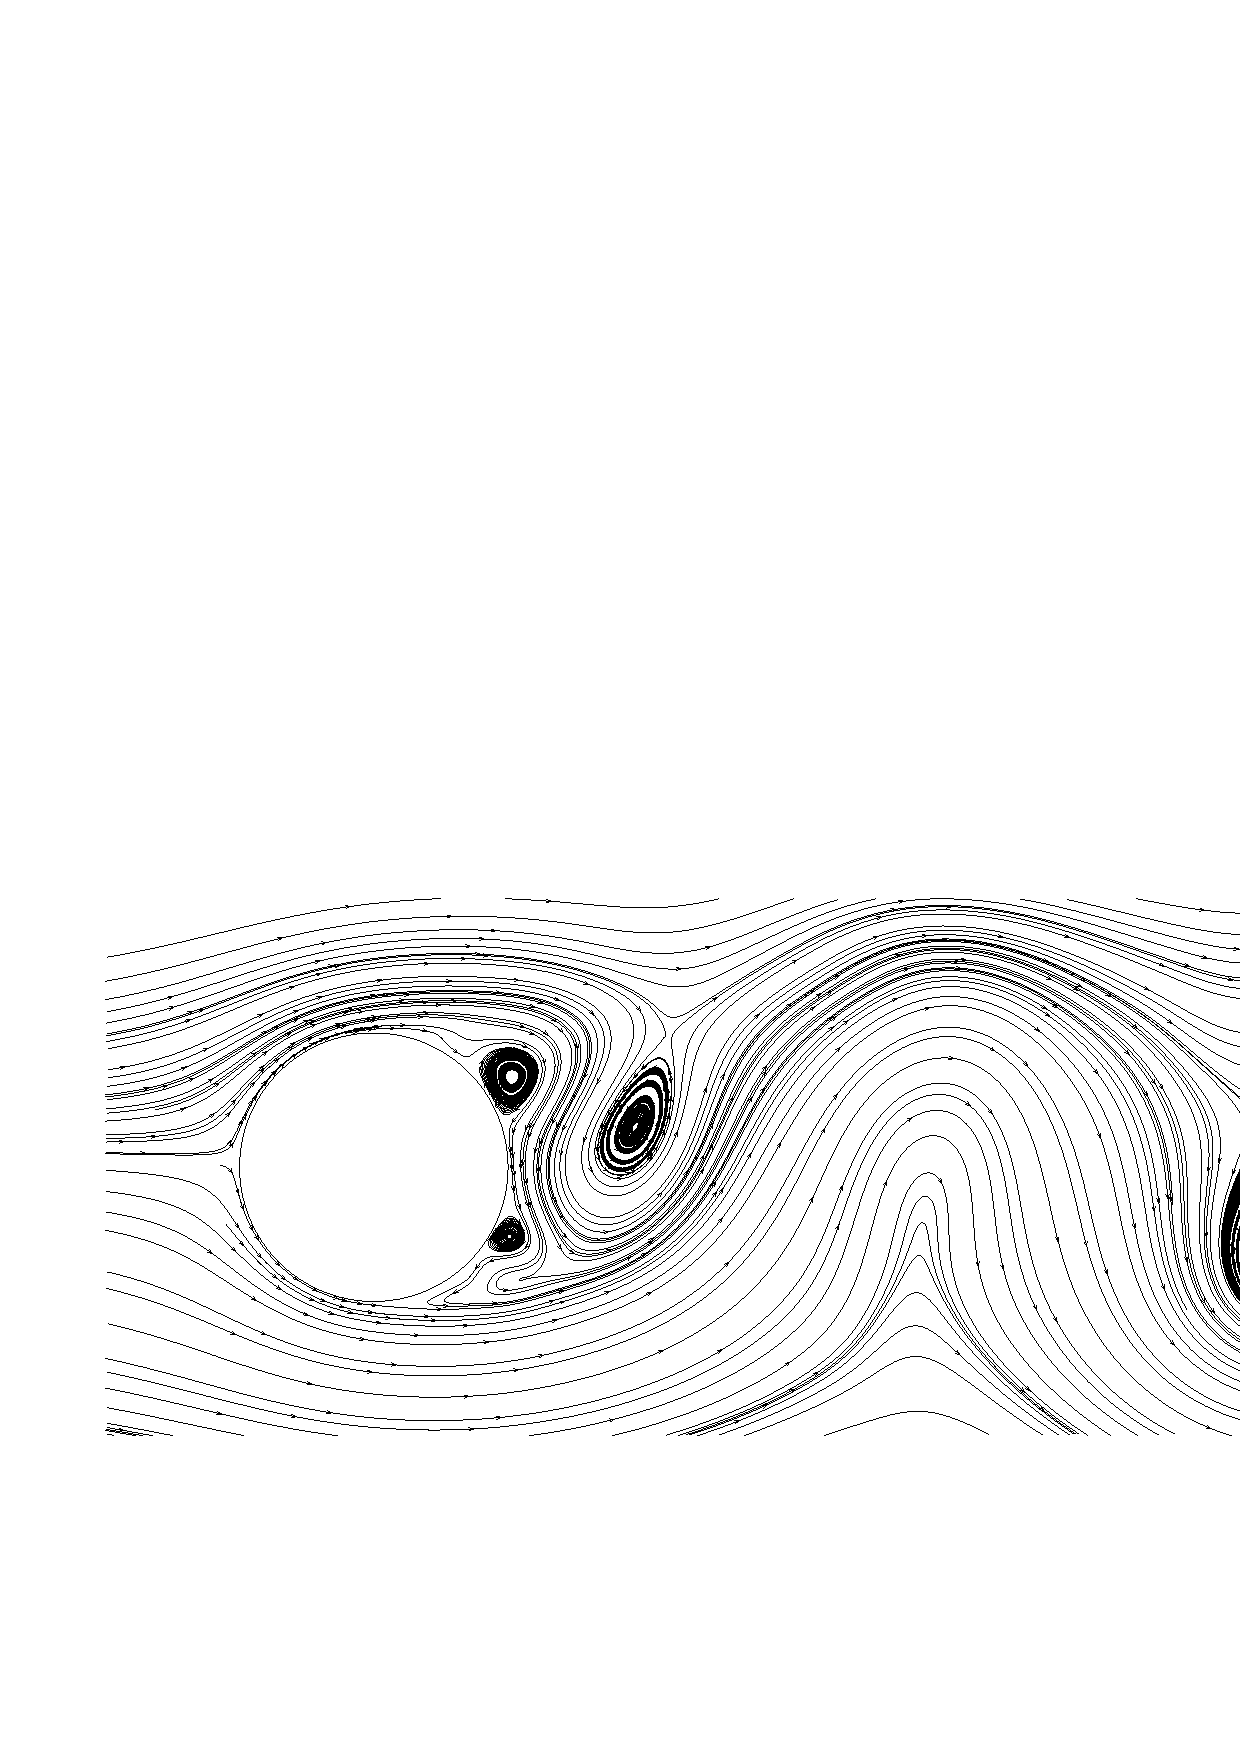
\includegraphics[width=45mm,clip=t]{CHAP_NONLIN/FIGURE/cim1.pdf}
        \\
         Time 4 & Time 5 & Time 6
       \end{tabular}}
  \end{tabular}
 \end{center}
 \vspace{-5mm}
 \caption{Circular cylinder. Instantaneous particle traces}
 \label{cil_sol1.fig}
\end{figure}
%

 Figs. \ref{cil_sol1.fig} reports the instantaneous
 particle traces in six instants over a cycle (the seventh position would be
 equivalent to the first) for two different $Re_d$.
 The shedding of the vortex is evident as well as the mechanism of their formation
 with a vortex merging. This is evident in Fig. \ref{cil_sol1.fig}a between instants
 3 and 4, and 6 and 1.
 It is worth to note the different pattern followed by the vortices for the two
 Reynolds number under consideration. For $Re_d= 400$ the
 shedding structure is well organised while for $Re_d= 4,000$
 the inertial forces play a more important role in the wake flow with formations
 of large recirculation bubbles which are propagated with small dissipation.
%
